\graphicspath{{Images/SVAs/}}

\chapter{SOFT VOXEL ACTUATORS: HYDROGEL BUILDING BLOCKS FOR BOTTOM UP ASSEMBLY OF SOFT ROBOTS}
\label{chap:SVAs}
Soft continuum manipulators are suitable for safe interaction with unstructured environments due to their compliance and theoretically infinite degrees of freedom (DOF). However, since current soft actuators resist miniaturization, using a large number of them to activate each DOF in a minaturized soft continuum manipulator has remained a challenge. This results in primitive miniature manipulators which have limited functionality. Here, we use a bottom-up voxel-based design and manufacturing methodology to integrate more actuators in soft robot manipulators while maintaining the small footprint of resulting robots. To solve challenges with miniturizing soft actuators, we introduce soft voxel actuators (SVAs) -- an active voxel actuated by electrical stimulus -- that resembles a group of muscle fibers (fascicles) in size, force production capacity and type of activation stimulus. We report the manufacturing method of SVAs, their frequency bandwith, and their static and dynamic force production capacity. We then show the advantages of the voxel-based methodology by assembling 4.5$\times$ 4.5$\times$4.5\,mm$^3$ SVAs weighing only 100\,mg into a miniature soft, continuum robotic manipulator with 16 DOFs in a 10$\times$40$\times$4.5\,mm$^3$ footprint. The arrangement of SVAs in this manipulator is inspired by the the arrangement of muscle fascicles in an octopus arm. We demonstrate the superiority of the SVA-based manipulator over conventional manipulators in interacting with unstructured environment. 
\section{Background}
\begin{figure*}[t]
      \centering
      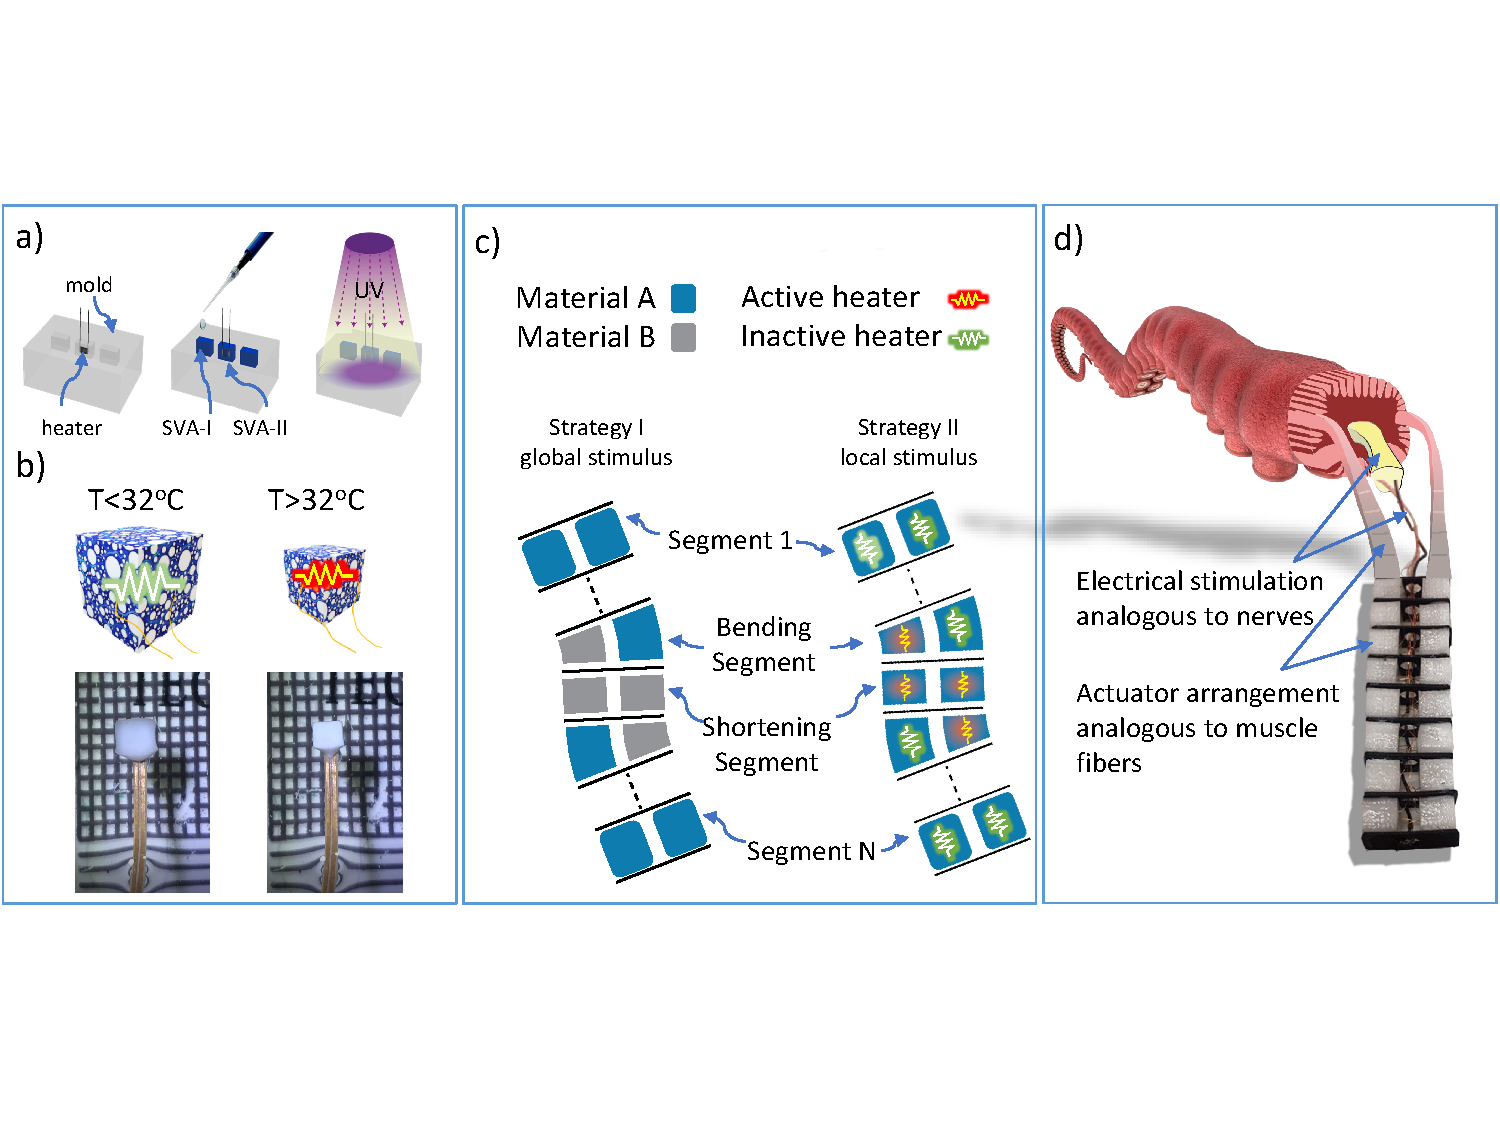
\includegraphics[width=\textwidth]{concept4.pdf}
      \caption[Soft Voxel Actuators (SVAs)]{\textbf{Soft Voxel Actuators (SVAs).} A: SVA manufacturing steps, B: a SVA in its actuated and unactuated staes C: The voxel-base design and manufacturing methodology based on electrically addressable SVAs has made possible the creation of miniature continuum manipulator with 16 DOFs.}
      \label{fig:conceptSVA}
\end{figure*}
Inspired by biology, soft robot developers try to utilize the advantages inherent in soft, compliant matter to achieve safer interaction with unstructured environments.  
While the applications of small-scale soft robots have been demonstrated or envisioned by many research groups \cite{Hines2017}, miniature and micro-scale soft robots have matured more slowly than their  macro-scale counterparts. The majority of soft robots utilize rigid components such as motors and pumps that are difficult to downscale \cite{Majidi2019} and therefore, manufacturing small-scale soft actuators has remained a bottleneck in the development of miniaturized soft robots. Smart, soft materials have shown promise in solving some of these challenges \cite{Steele2018, Stuart2010, White2013}; these smart materials react to changes in pH, temperature, or electric, magnetic and light fields by producing stress/strain fields in the material to create motions such as bending, twisting, or elongation. These motions have been harnessed for applications such as drug delivery \cite{ghosh2017}, micro-grippers \cite{shintake2018}, or other primitive robots~\cite{Ionov2014}. %such as dielectric elastomer actuators (DEAs), ionic polymer-metal composites (IPMCs) and stimuli-responsive hydrogels 
%Performing sophisticated tasks while interacting with unstructured environments requires independent actuation of many degrees of freedom in coordination with each other. Smart soft materials have nearly infinite active degrees of freedom meaning each infinitesimal region can be considered as a virtual actuator. The nature of stimuli such as PH, magnetic fields or electric fields however, prevents systems of actuators from being individually addressed. As a result, these materials are often activated globally, meaning that all the virtual actuators in the material are activated at the same time using a stimulus that acts globally on the entire system \cite{ceylan2017mobile}. Structured light has been shown to address this issue by independently addressing more degrees of freedom in smart soft materials \cite{palagi2016structured}. This method, however has other limitations, as the light cannot reach the interior of material volumes to excite regions that are out of sight. The most intuitive and bio-inspired stimulation technique is electrical stimulation, which is closest to electrical potentials used in the nervous systems of living animals. Common materials that can be activated by electrical potentials or currents include DEAs, LCEs and IPMCs\cite{carpi2011dielectric}. Due to the complexity of manufacturing these material systems, miniature robotic mechanisms in the literature that use these materials [] have demonstrated only a few degrees of freedom. Utilizing higher number of virtual actuators inherent in these materials can become challenging. DEAs, for example, require high voltages which in turn requires additional, often bulky electric components; IPMCs produce only bending motions and exhibit other non-ideal behaviors such as Back Relaxation \cite{annabestani2016restraining}. Robots resulting from these materials have remained primitive in the sense that they can only perform simple, context-specific tasks that they are designed for. When the task changes during their operation-- a case which often happens in unstructured environments-- these robots fail.  
%
%
%Temperature responsive hydrogels, by contrast, can be stimulated electrically using Joule heating \cite{yu2013electronically}. The electrical stimulation can be confined to micron-sized regions making it possible to individually address more virtual actuators in the material \cite{richter2009optoelectrothermic}. However, they are usually sluggish in their response especially at larger scales, making them unsuitable for many robotic applications. We have previously reported solving the problem of slow response of temperature responsive hydrogels \cite{emami2019}. Based on that result, we now present a novel, soft actuator along with a design methodology for solving some of the challenges related to miniaturizing soft actuators and the resulting soft robots. These actuators, which we called soft voxel actuators (SVAs), are made using temperature-responsive hydrogels and electrically activated by Joule heaters. Our design and manufacturing approach is to consider the entire body of a soft robot as a collection of smaller units called voxels. %ach SVA is the physical realization of the virtual actuators inherent in smart soft materials.
%Assembly of these voxels results in a soft robot with many individually addressable degrees of freedom. %Since each voxels is an individually-addressable actuator, the resulting robot contains many degrees of freedom that can be controlled electrically. %In addition to material properties of tmeperature-responsive hydrogel used in OUR SVAs, the performance of the actuators is also dependent on the shape, and working conditions of the actuator. Therefore, in this paper, 
%We have characterized the force and stroke of each SVA and proposed bio-inspired configurations (Figure~\ref{fig:conceptSVA}) for assembling SVAs in ways that results in general miniaturized mechanisms capable of performing more sophisticated tasks than found in current literature. We can demonstrate that SVAs can be used in a bottom-up approach to build miniature continuum manipulators with hyper-redundant DOFs. This miniature manipulator is 10$\times$ 40 $\times$ 4.5\,mm$^3$ and has 16 DOF making it robust in creating complex interactions with unstructured environments.  
%\textcolor{red}{This paper demonstrates how SVAs support the development of soft, miniature continuum, robotic arms  -- a challenge difficult to realize with competing technologies}.
%
%\section{Soft Voxel Actuators (SVAs)}
%In computer-based modeling or graphic simulation, the word ``voxel'' typically refers to 3-dimensional (3-D) units used to represent shapes in 3-D space; they are the 3-D equivalent to pixels, which are used for representing objects and images in 2-D  space \cite{sossou2019design}. The recent use of physical voxels in additive manufacturing, using passive and often rigid materials,  has been demonstrated in literature and patents \cite{hiller2009design}. However, the physical realization of soft voxels using stimuli-responisve materials that can act as individually-addressable actuators has not yet been demonstrated. Manufacturing and characterization of such actuators as simple building blocks for use in a bottom-up approach to construct complex robotic systems is demonstrated herein.
%
\section{SVA Fabrication}
SVAs were made through a molding process in the form of cubes of different dimensions, as shown in Figure~\ref{fig:Manufac}. The molds were made with PDMS (Sylgard 184, Dow Corning) because of its transparency to UV light and its elasticity, so that the cured hydrogel may be easily and fully demolded without breaking. Since the hydrogel swells from its molded dimensions upon soaking in water, the dimensions of the molds were selected to be smaller than the required dimensions of the actuator. A nylon mold was prepared using a 3D printer (Markforged, M2) and was used to create the PDMS mold. For selecting Joule heaters, several types of resistive heaters were examined to find the optimum one in terms of manufacturability, durability, and compatibility with other electronic components. Surface mount resistors have all the required properties and therefore were chosen as the heating elements (Figure~\ref{fig:Manufac}). The value of the resistor was chosen such that it produced enough heat to set the equilibrium temperature of the SVA from room temperature ($25^{o}C$) to above the transition temperature of the hydrogel ($32^{o}C$) and cause it to shrink when a 3.7 $V$ supply voltage was connected to it. This actuation voltage was chosen to be compatible with many commonly used microcontrollers that are available on the market. In this paper, we have used surface mount 
(SMD) thick film resistors with a resistance of 10~ohms which is shown in Figure~\ref{fig:Manufac} along with its dimensions.  For manufacturing each SVA, a resistor (Joule heater) was positioned inside the mold using an XYZ manual stage (Figure~\ref{fig:Manufac}) before the precursor solution was added and cured along with the gel. The heater was placed at a position equidistant from each side of the mold so that the entire volume of the gel was heated as uniformly as possible to avoid undesired nonuniform deformation of the actuators. PNIPAAm precursor solution was poured into the molds using pipettes while the resistive heater was held in place using grippers. A UV LED (UV 365nm, 10W, Chanzon, China) was used for curing the gels. 

\begin{figure*}[h]
      \centering
      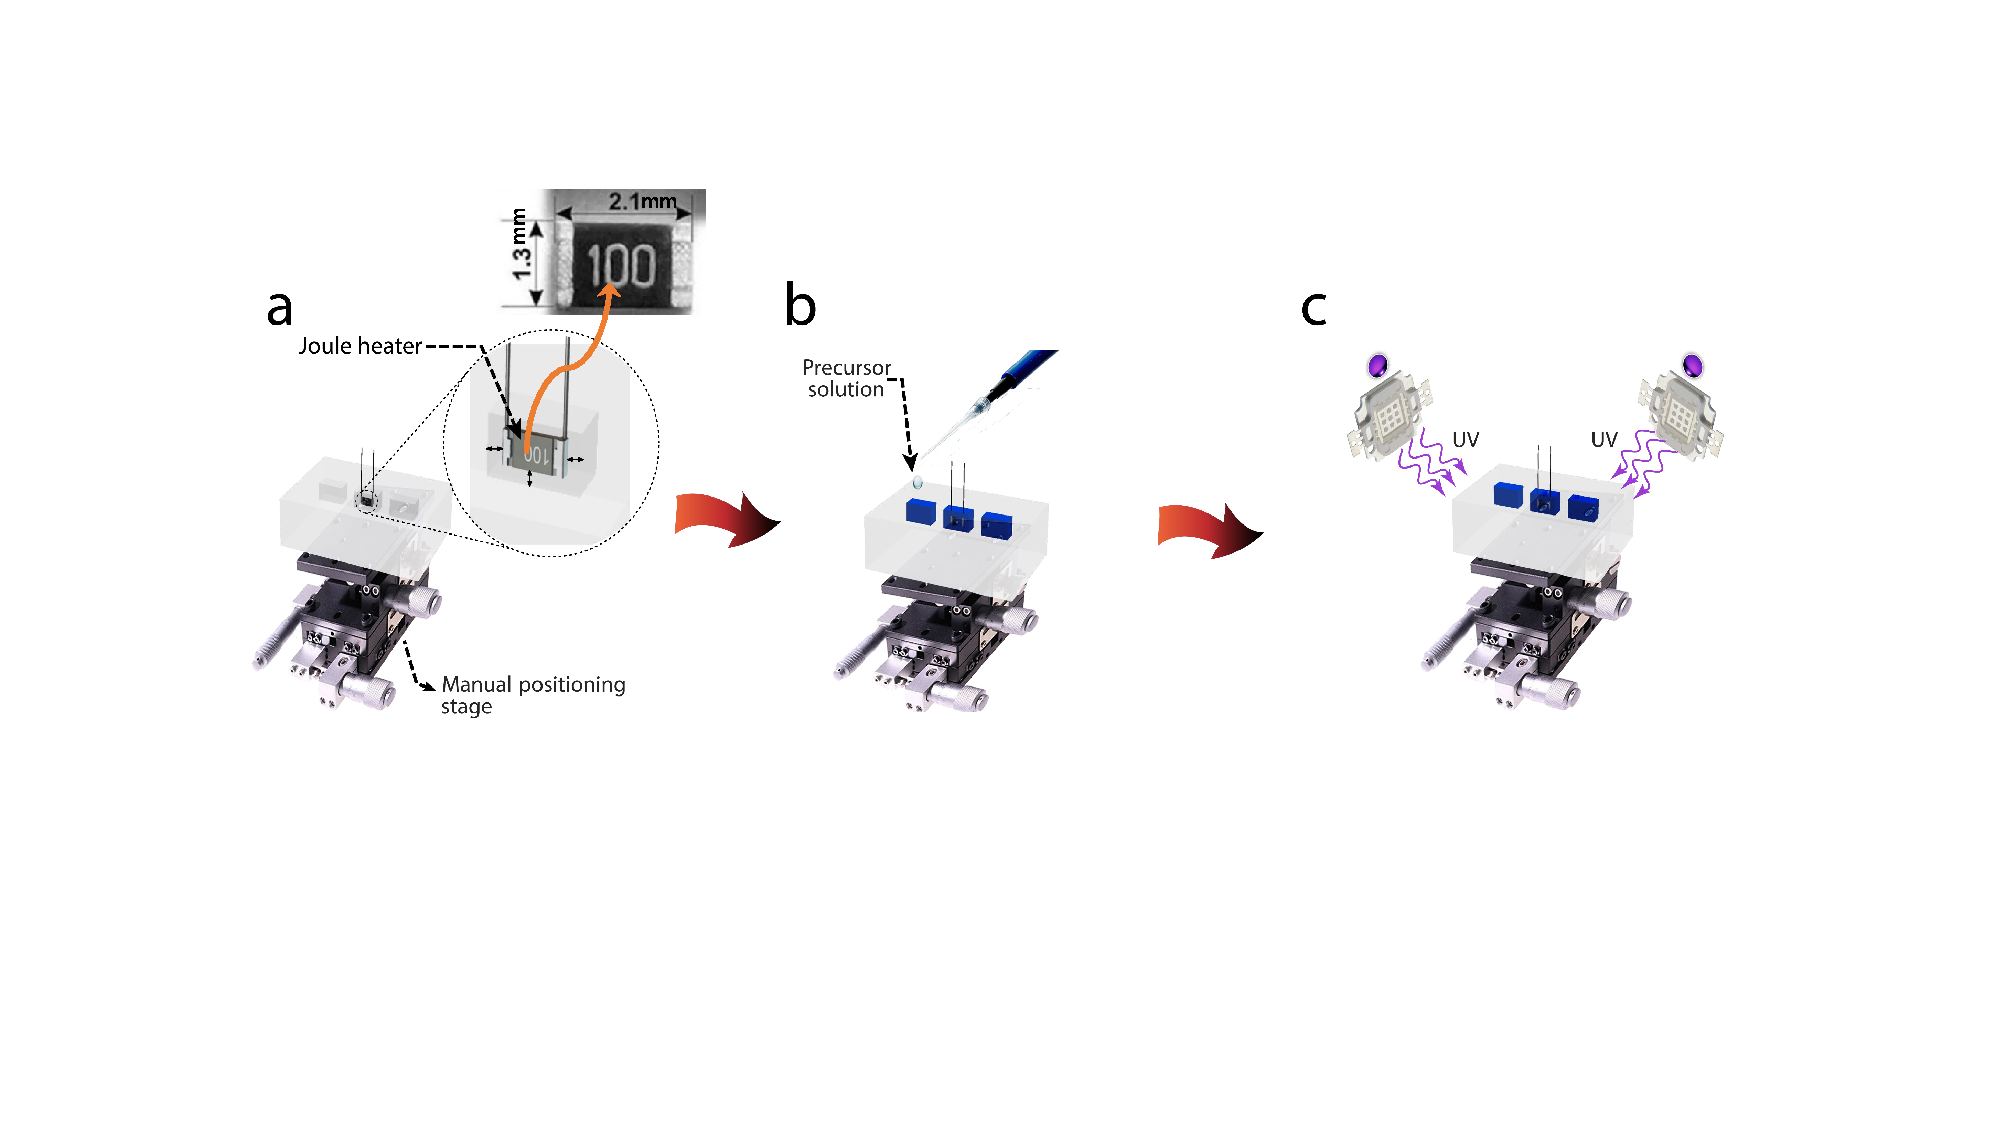
\includegraphics[width=\textwidth]{svaManufacturing.pdf}
      \caption[Steps for manufacturing SVAs]{\textbf{Steps for manufacturing SVAs.} A) A Joule heater (surface mount (SMD) thick film resistors with a resistance of 10 ohms) is placed in the PDMS mold using an XYZ manual stage. B) Precursor solution is added to the mold. C) Hydrogel is formed by curing the solution under UV light for 10 seconds.}
      \label{fig:Manufac}
\end{figure*}

\section{SVA force measurements}
The force generated by an SVA was measured using a 100~g load cell and a load cell bridge amplifier (PhidgetBridge 1046_0B, Phidget, Canada) in the setup shown in Figure~\ref{fig:forceTestSetup}. The SVA was placed under the load cell, the joule heater was activated allowing the SVA to shrink to its minimum volume, and then the linear stage was lowered to bring the load cell in contact with the surface of the SVA as shown in Figure~\ref{fig:forceProcedure}. The interface between the load cell and the SVA was made from an acrylic plate. In force measurement tests where the SVA expands and pushes against the load cell, this plate just touches the surface of the SVA. In other tests where the SVA contracts, superglue was used to bind the acrylic plate to the SVA, so that the SVA pulled on the load cell as it contracted. The experiment is performed in a water bath at room temperature (25$^o$C). The load cell was calibrated while the acrylic plate was underwater but not touching the SVA. A two-point calibration method was used with a 50~g precision weight.

\begin{figure*}[h]
      \centering
      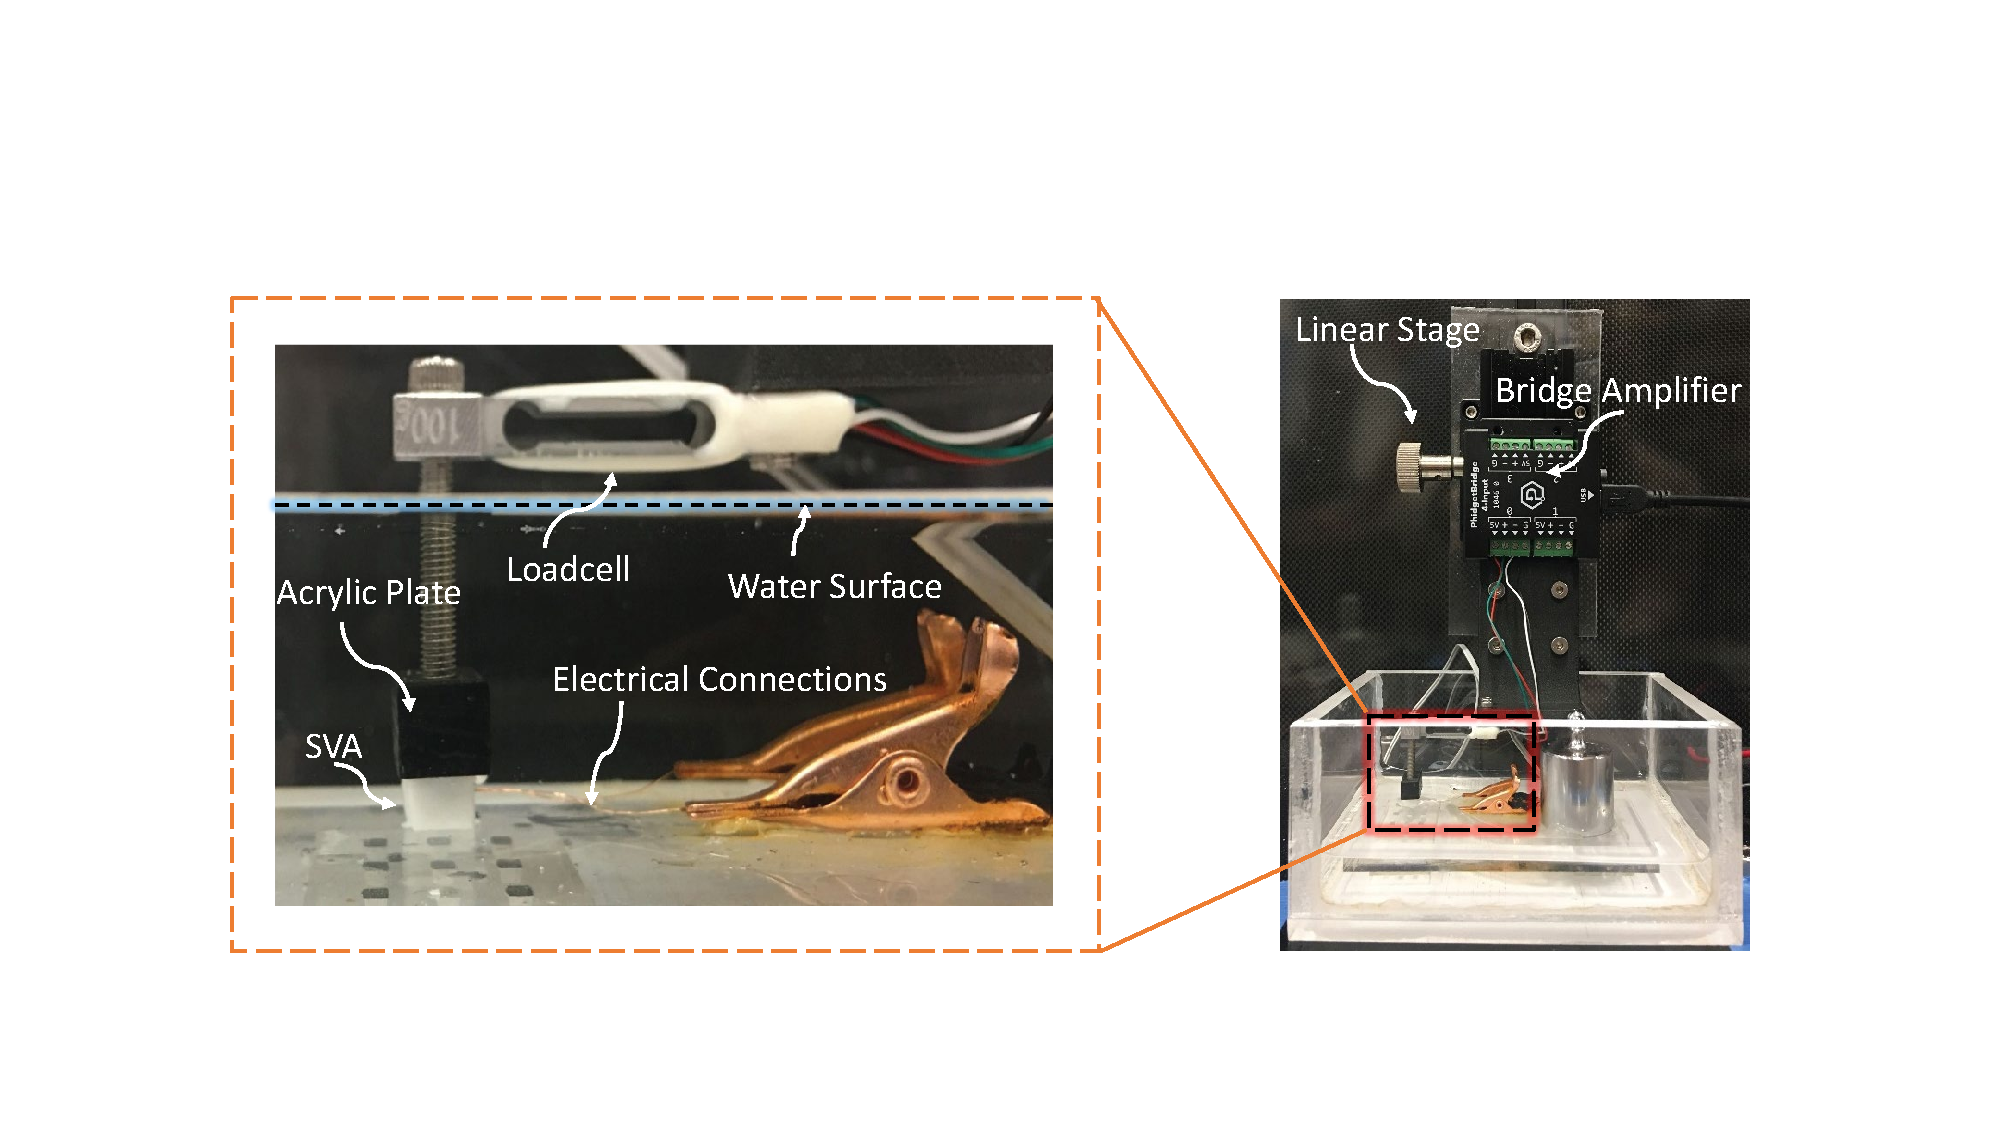
\includegraphics[width=\textwidth]{forceTestSetup.pdf}
      \caption[Force measurement test setup]{\textbf{Force measurement test setup.} SVA force is measured using a load cell and a bridge amplifier.}
      \label{fig:forceTestSetup}
\end{figure*}

\begin{figure*}[!h]
      \centering
      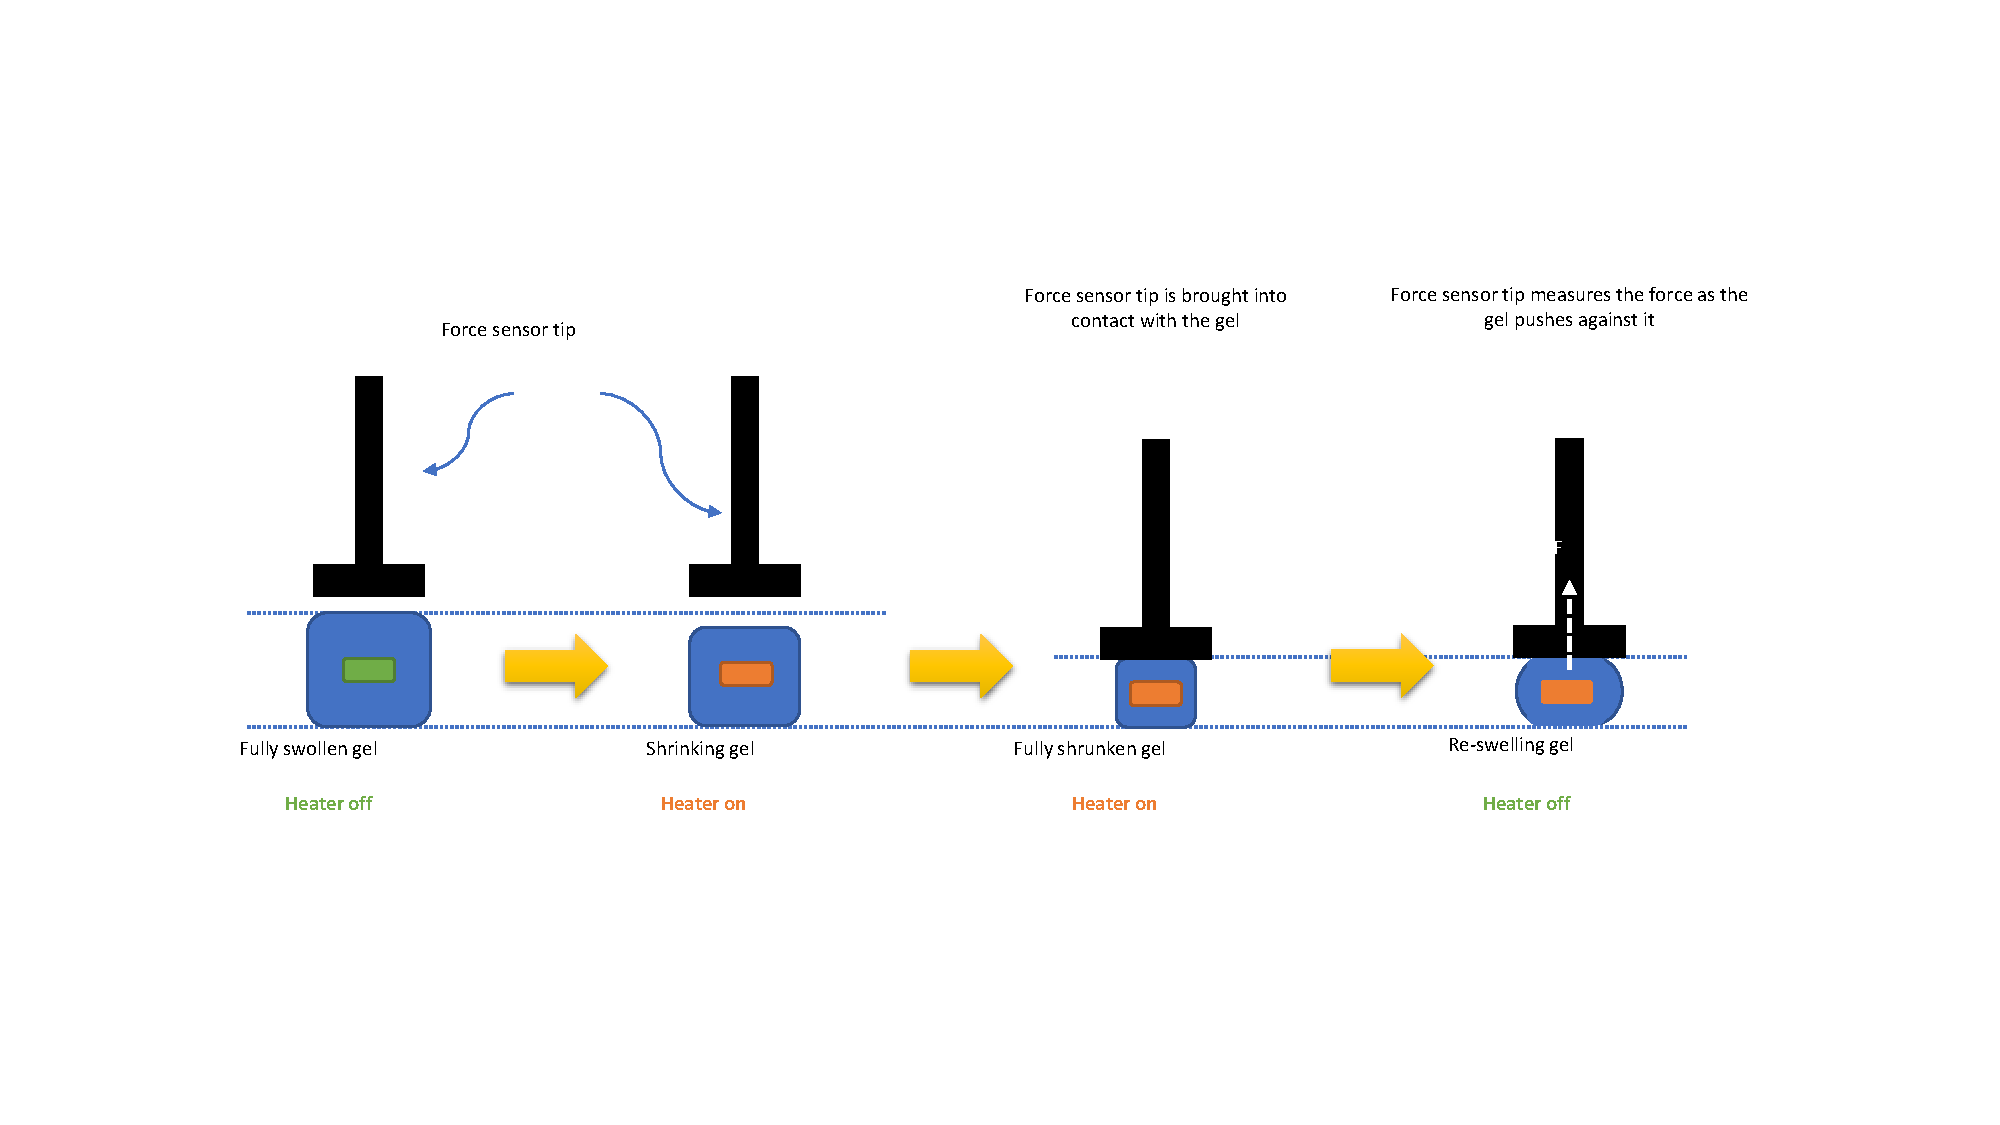
\includegraphics[width=\textwidth]{forceProcedure.pdf}
      \caption[Force measurement procedure]{\textbf{Force measurement procedure.} Steps of placing the sensor tip on the SVA for compressive force measurement.}
      \label{fig:forceProcedure}
\end{figure*}

the force produce by the SVA is depended on its material properties. Since the material properties of the hydrogels can be tuned by varying Figure~\ref{fig:svaForce}
\begin{figure}[!htb]
\centering
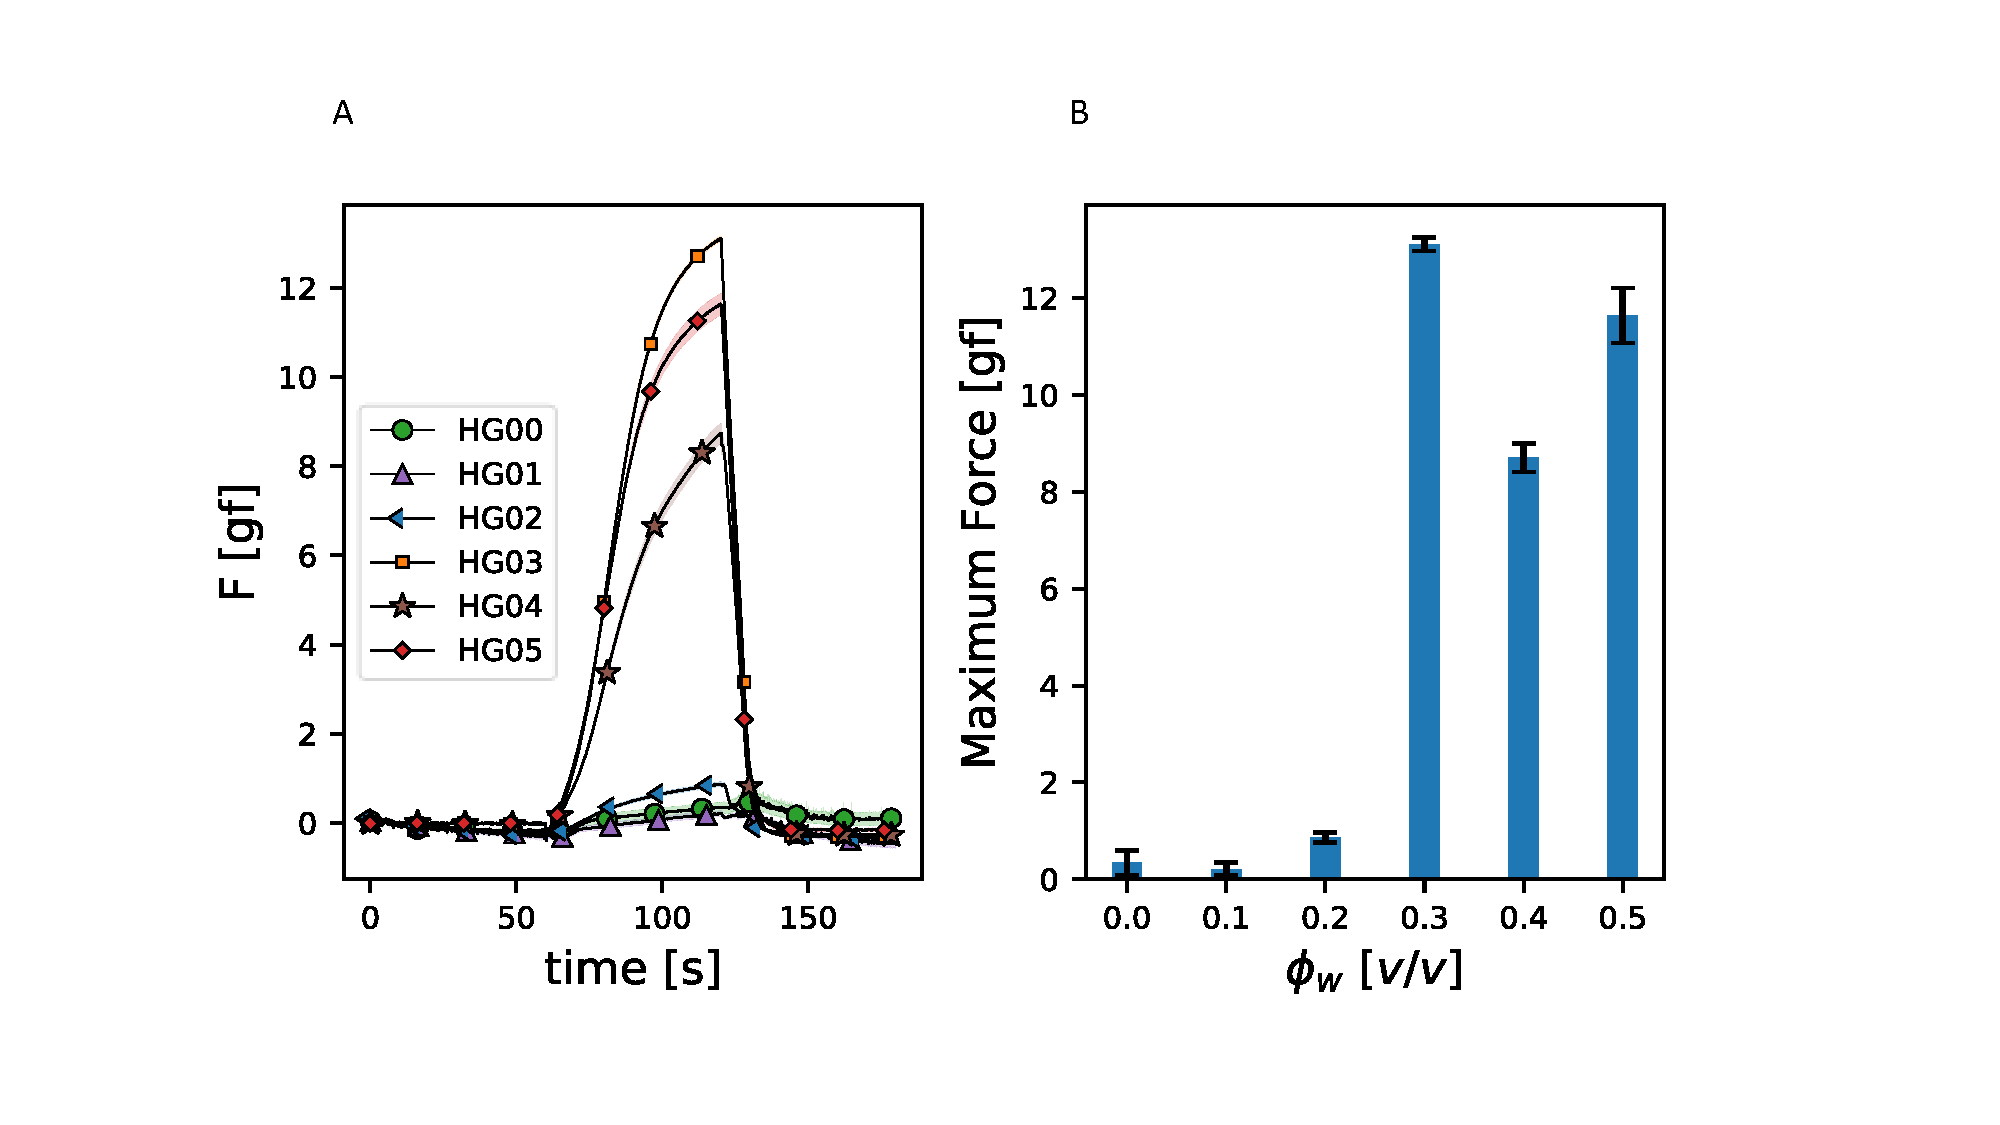
\includegraphics[width=\textwidth]{svaForce.pdf}
    \caption[Tuning the mechanical properties of SVAs]{\textbf{Tuning the mechanical properties of SVAs by varying water volume fractions $\phi_{w}$.} A) Force produced by a SVA as a function of time for different $\phi_{w}$. B) Maximum force produced by a SVA as a function of $\phi_{w}$. }
    \label{fig:svaForce}
\end{figure}

\section{SVA swelling ratio measurements}
Swelling ratio, a commonly studied property of hydrogels, is a measure of the ability of the gel to absorb water. Robotics applications which use fast responding hydrogels such as the one presented in this paper require a method of characterization of the hydrogel swelling ratio, to quantify volume changes in real-time in order to capture the volume changes that happen in short amount of time. We have developed a method that uses image processing techniques to measure the linear displacement produced by a SVA, as shown in Figure~\ref{fig:swellingTestSetup} S3. The volume change of a SVA results in the movement of a lever arm contacting the SVA, and the resulting vertical displacement of the tip of the lever arm is then measured. 

\begin{figure*}[!h]
      \centering
      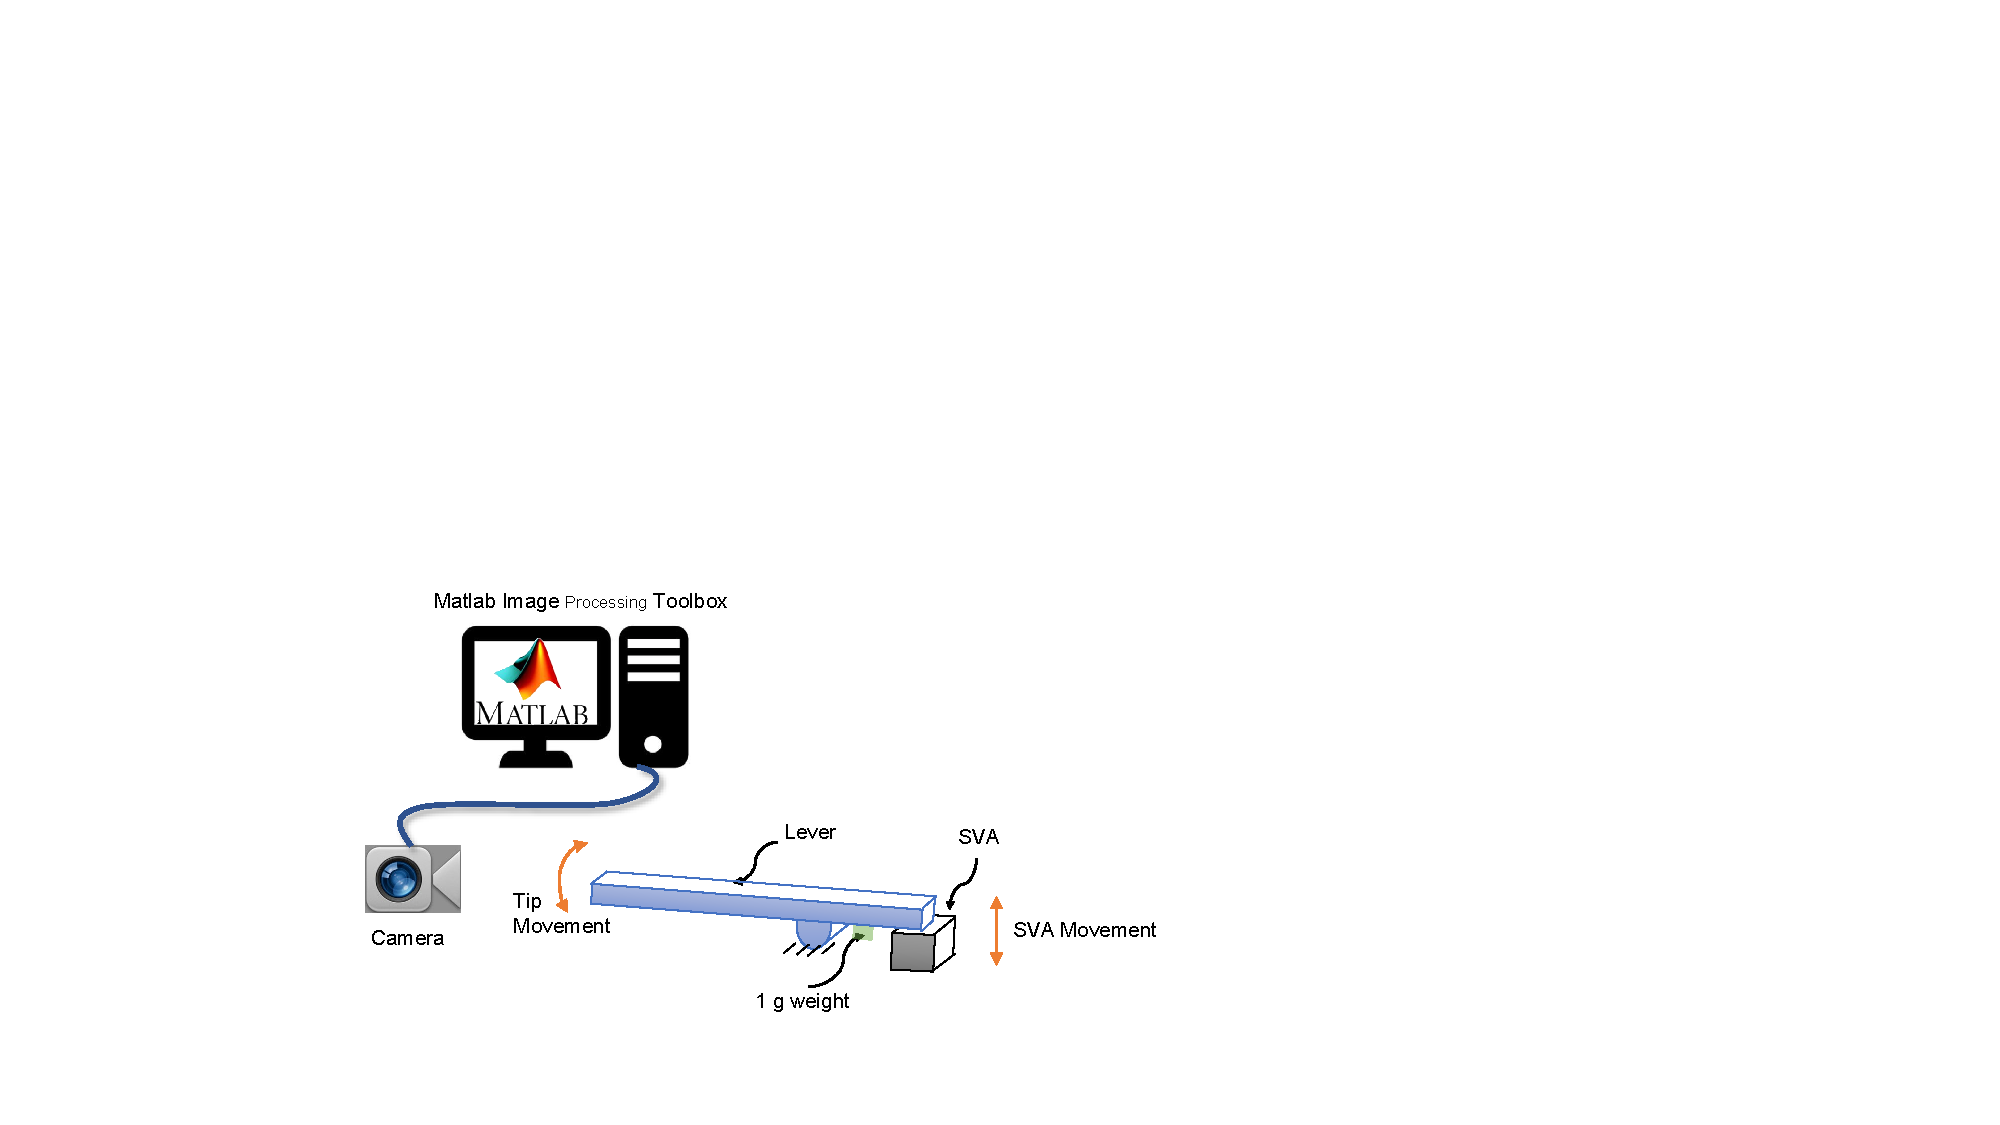
\includegraphics[width=\textwidth]{swellingTestSetup.pdf}
      \caption[SVA displacement measurement setup]{\textbf{SVA displacement measurement setup.} A camera is used to track the angular displacement of the tip of a lever arm, which is proportional to the vertical displacement of the SVA (assuming small displacements). The 1 g weight is affixed to the lever arm to ensure that the lever is always in contact with the SVA.}
      \label{fig:swellingTestSetup}
\end{figure*}

Since this vertical displacement is small, the curve followed by the tip can be approximated by a straight line and is proportional to the vertical displacement of the SVA. A marker on the tip is tracked by a Logitech C930e USB Webcam, which can stream HD 1080P quality video. This webcam is compatible with the MATLAB Image Acquisition and Image Processing Toolboxes. In each test, a checkerboard was placed in the same plane as the marker on the tips of the lever arm. This checkerboard had black and white squares of dimensions 2 mm × 2 mm and was used to estimate the calibration factors (mm/pixel) in the x and y directions. Since we used contrast-based filtering, the marker color was selected to be white whereas the color of the background was chosen to be black to create a clear contrast against the background. We also used MATLAB’s Camera Calibration Toolbox to compensate for the lens distortions. The experiment is performed in a water bath at room temperature ($25^{o}C$).


\section{Dynamic Mechanical Analysis (DMA) tests}
Each hydrogel prepolymer recipe was cast into a dogbone shape with 2.5 mm thickness and 1.5 mm neck width. This was done by pouring the prepolymer solutions into PDMS molds with the specified dogbone dimensions and polymerizing them under UV light for 15 seconds. The dogbones were then removed from the PDMS molds and immersed in a large container of DI water to remove excess monomer and DMSO. To measure Young’s modulus, the dogbones were loaded into a Dynamic Mechanical Analyzer machine (TA Instruments DMA850) and subjected to a strain rate of $8\% min^{-1}$. The Young’s modulus was obtained from the slope of this stress-strain measurement (Figure~\ref{fig:DMA}). In addition, we have performed cyclic strains tests using the DMA device to study any material behavior changes over time (Figure~\ref{fig:stressCycle}).

\begin{figure*}[!th]
      \centering
      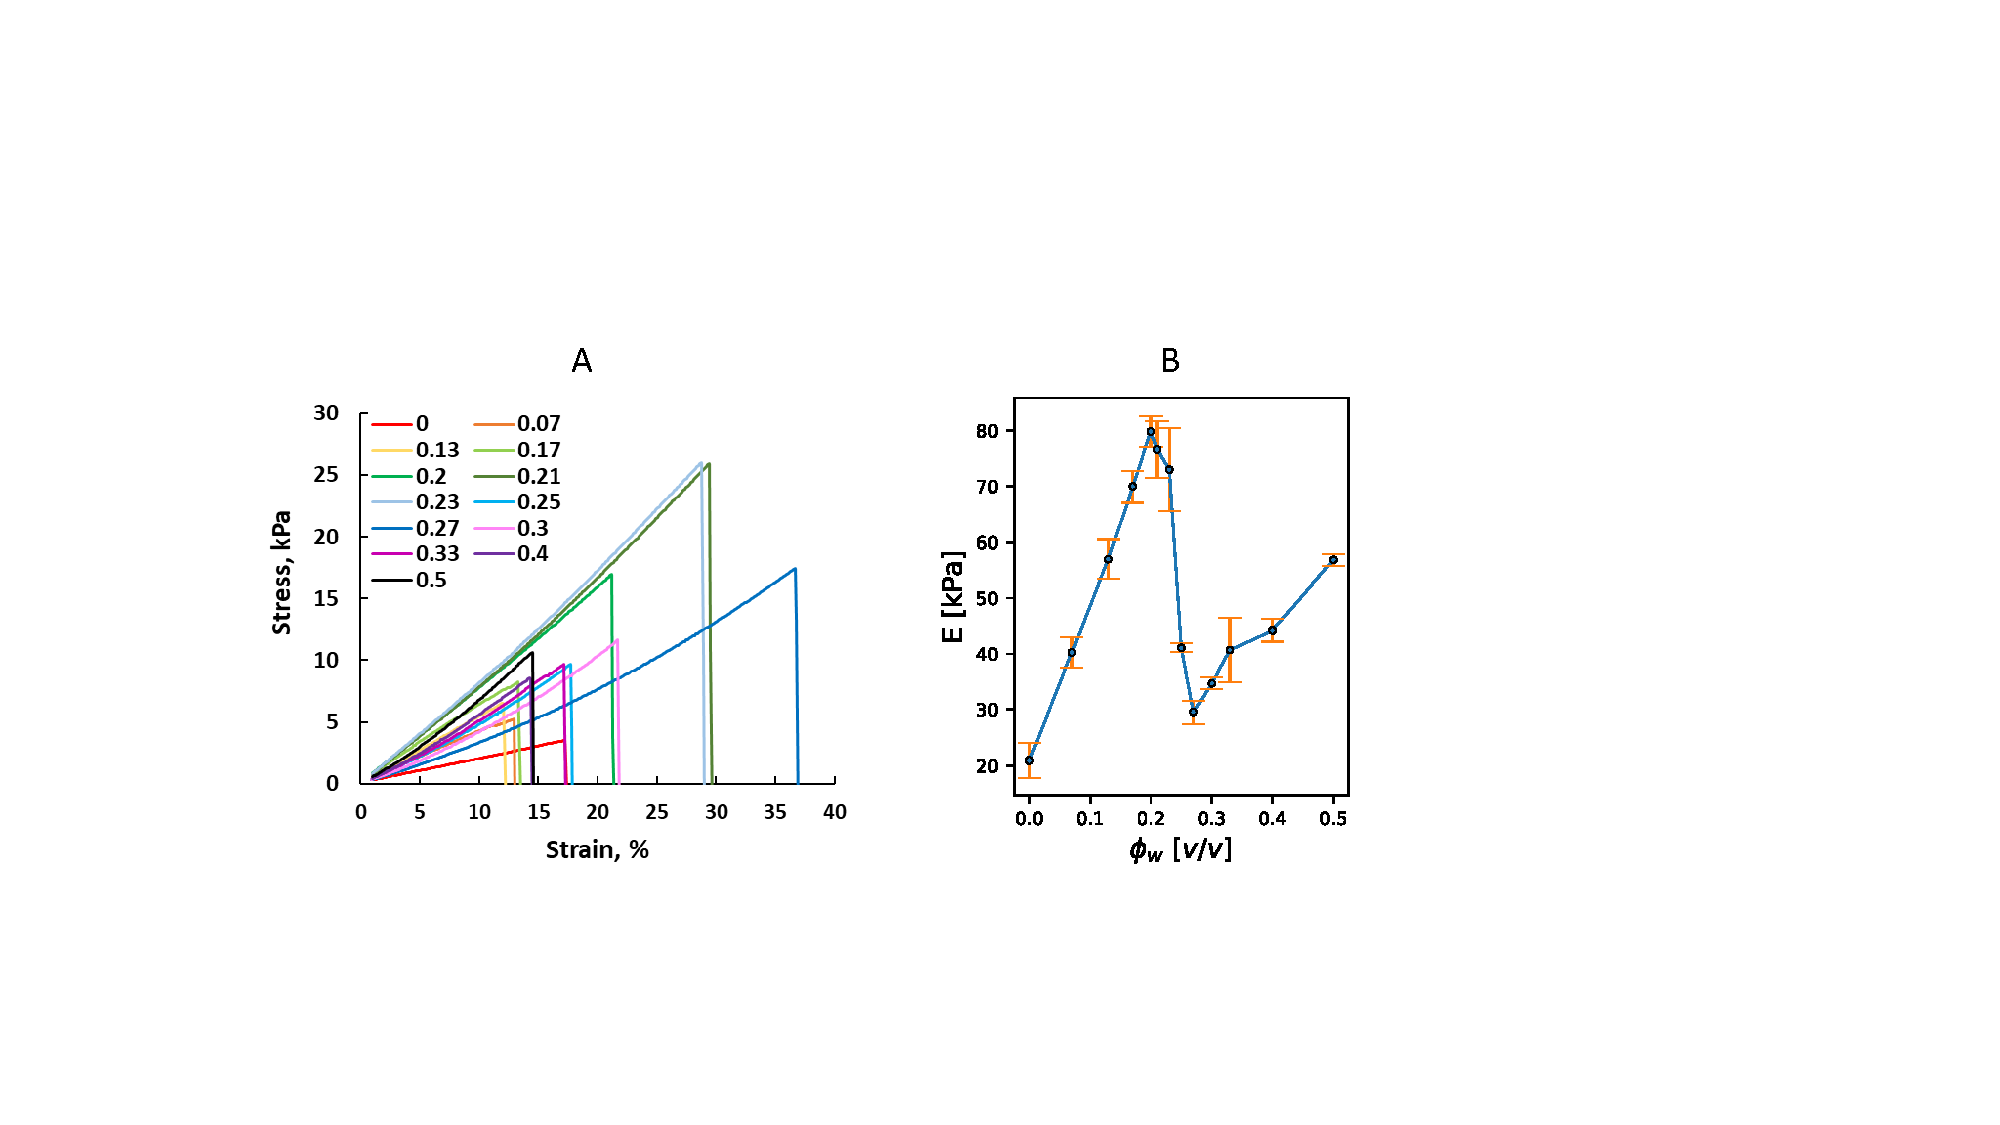
\includegraphics[width=\textwidth]{DMA.pdf}
      \caption[Dynamic mechanical analysis (DMA)]{\textbf{Dynamic mechanical analysis (DMA) test.} stress-strain curves (left) and derived Young’s modulus of the hydrogels as a function of water volume fraction ($\phi_{w}$).}
      \label{fig:DMA}
\end{figure*}

\begin{figure*}[!th]
      \centering
      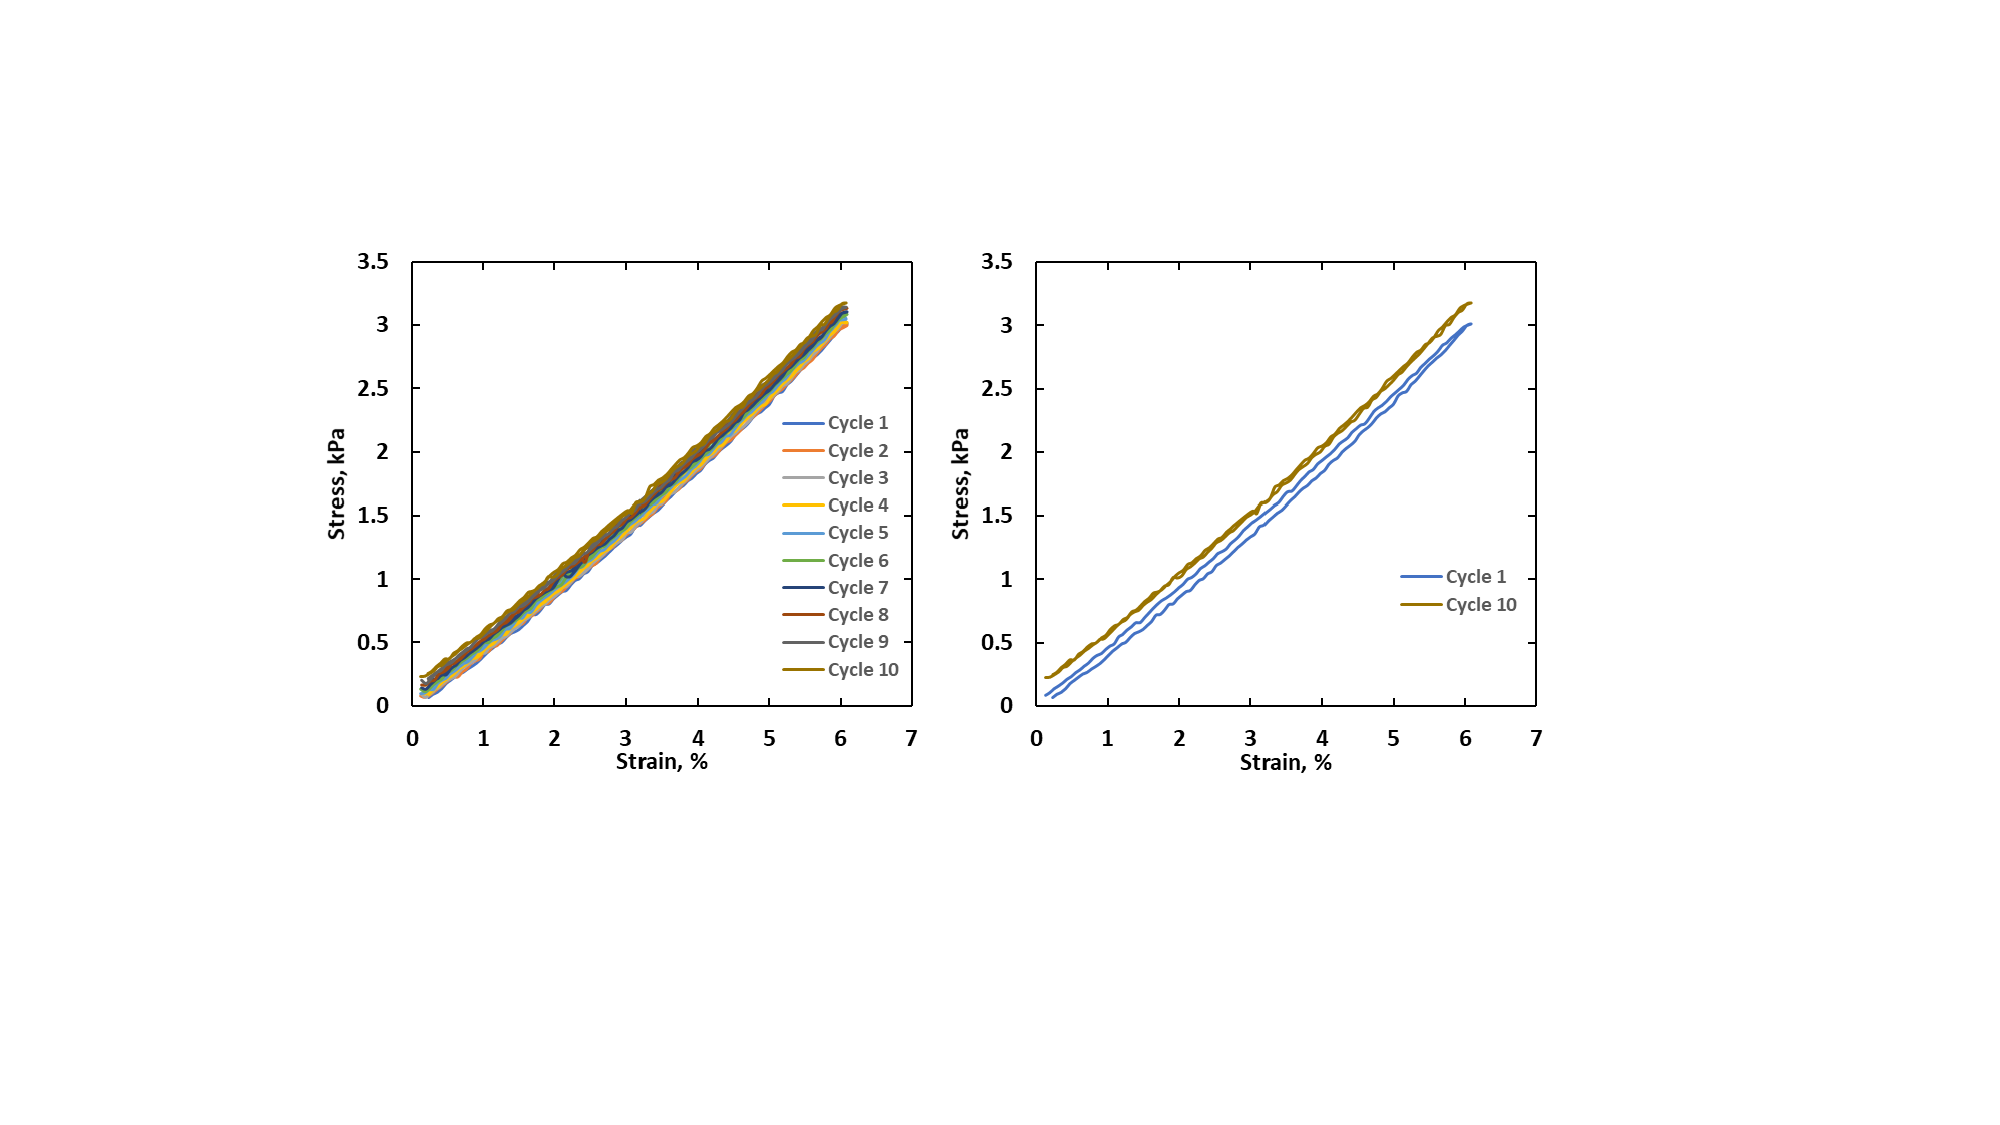
\includegraphics[width=\textwidth]{stressCycle.pdf}
      \caption[Cyclic load test]{\textbf{Cyclic load test.} Stress-strain cycle test of HG03 ($\phi_{w}=0.3$) dogbone, demonstrating stability over 10 cycles (left). Stress-strain curves of Cycle 1 and Cycle 10, demonstrating a gradual shift upwards, due to drying-induced stiffening (right). A strain rate of $20\% min^{-1}$ is used to mitigate the effects of drying-induced stiffening.}
      \label{fig:stressCycle}
\end{figure*}

\section{Crosslink density using Flory theory}
The Flory-Rehner rubber elasticity theory provides a simple approach for calculating crosslink density from swelling measurements. The equation is as follows :
\begin{align}
	-[\ln⁡(1-\nu_2)+\nu_2+\chi_1 (\nu_2 )^2 ]=V_1 n[(\nu_2 )^{(\frac{1}{3})}-\frac{\nu_2}{2}]
\end{align}
%-[ln⁡(1-ν_2 )+ν_2+χ_1 (ν_2 )^2 ]=V_1 n[(ν_2 )^(1/3)-ν_2/2]
%\ln(w)
In the above, $\nu_{2}$ represents the volume fraction of the polymer in the hydrogel, $\chi_{1}$  represents the Flory-Huggins interaction parameter for PNIPAAm-water  which is equal to 0.5,  $V_{1}$ represents the solvent (water) molar volume ($18~cm^3~mol^-1$), and n represents the density of linear polymer segments bound by crosslinks on both ends. $\nu_{2}$ can be expressed in terms of the polymer volume ($V_polymer$) and gel volume ($V_gel$), as follows:
\begin{align}
	\nu_2=\frac{V_{polymer}}{V_{gel}} =\frac{(\frac{{m_polymer}}{\rho_{polymer}})}{V_{gel}} 
\end{align}

$V_{gel}$ can be measured directly from the dimensions of a regular-shaped hydrogel; m_polymer is the dry mass of this hydrogel after freeze-drying. The density of the polymer ($\rho_{polymer}$) can be measured via the following volume relationship:

\begin{align}
	V_{gel}=\frac{m_{water}}{\rho_{water}} +\frac{m_{polymer}}{\rho_{polymer}} 
\end{align}

This can be re-written in the following:
\begin{align}
	\rho_{polymer}=\frac{m_{polymer}}{(V_{gel}-\frac{m_{water}}{\rho_{water}})}
\end{align}

Here, $m_{water}$ represents the mass of the wet hydrogel minus $m_{polymer}$. With these relationships, $\nu_{2}$ for photo- and thermo-polymerized HG03 PNIPAAm can be calculated, and hence $n$ can be obtained. Furthermore, the average molecular weight of crosslinked polymer segments $(M_{c})$ can also be calculated using the following modified equation, assuming the hydrogel is composed of a completely continuous polymer network:

\begin{align}
	-[\ln⁡(1-\nu_{2} )+\nu_{2}+\chi_{1} (\nu_{2} )^{2}]=(\frac{V_{1}}{(\overline{\nu} M_{c})})[(\nu_{2} )^{(\frac{1}{3})}-\frac{\nu_{2}}{2}]
\end{align}

Here, $\overline{\nu}$ represents specific volume of the polymer in the hydrogel, represented by the following:
\begin{align}
\overline{\nu}=\frac{V_{gel}}{m_{polymer}} 
\end{align}
Table~\ref{table:flory} lists the key values of relevant properties calculated with this method.

\begin{table}[htbp]
\centering
\captionsetup{justification=centering}
\caption{Values of mass fraction of water, volume fraction of polymer, $n$, and $M_{c}$ for photo- and thermo-polymerized HG03 hydrogels.}\vspace{-0.25cm}
\begin{tabular}{c c c}
\hline
\hspace{-2mm}  & Photo & \hspace{-2mm} Thermo\\
%\hspace{-2mm} (mm) &  trajectory   & (g)  & (mm)& (mm)& (mm) & \hspace{-2mm}$\%$\\
\hline
\hspace{-2mm}$m_{water}$ & 0.87    & \hspace{-2mm}0.85\\
\hspace{-2mm}$V_{Polymer}$ & 0.26  & \hspace{-2mm}0.27\\
\hspace{-2mm}$n(\frac{mol}{cm^{3}})$ & $7.56 \times 10^{-4}$ & \hspace{-2mm}$9.37 \times 10^{-4}$\\
\hspace{-2mm}$M_{c}(\frac{g}{mol})$ & 149       & \hspace{-2mm}140\\
%\hspace{-2mm}9 & Half Ellipse      & - & 0.129 & 0.058 & 0.132 & \hspace{-2mm}9.8\\
%\hspace{-2mm}9 & Quarter Ellipse   & - & 0.161 & 0.061 & 0.171 & \hspace{-2mm}12.8\\
%\hspace{-2mm}25 & Ellipse          & 1 & 0.140 & 0.022 & 0.144 & \hspace{-2mm}8.9\\
%\hspace{-2mm}25 & Ellipse          & 2 & 0.162 & 0.021 & 0.162 & \hspace{-2mm}10.1\\
%\hspace{-2mm}25 & Ellipse          & 3 & 0.164 & 0.022 & 0.164 & \hspace{-2mm}10.2\\ 
\hline
\end{tabular}
\label{table:flory}
\vspace{-4mm}
\end{table}

\section{Scanning Elecron Microscope (SEM) Imaging}
To prepare SEM samples, each hydrogel prepolymer recipe was photopolymerized under UV light in a 1~mm$\times$5~cm$\times$7~cm PDMS mold to form sheets. After rinsing in DI water to remove DMSO and excess monomer, the sheets were cut into $1~mm$ thick slices. These slices were immersed in liquid nitrogen to instantly freeze and then immediately placed in a freeze-drier for 24 hours to remove the ice. The freeze-dried hydrogel slices were then imaged under SEM after sputtering a $5-10~nm$ layer of gold on them. The SEM images for hydrogels with different solvent ratio is shown in Figure~\ref{fig:compiledSEM}

\begin{figure*}[!th]
      \centering
      \includegraphics[width=\textwidth]{compiledSEM.pdf}
      \caption[SEM images]{\textbf{SEM images of the hydrogel microstructure.} The numbers indicate the water volume fraction ($\phi_w$). The scale bars are 10$\mu$m and 1$\mu$m for the low and high magnifications, respectively.}
      \label{fig:compiledSEM}
\end{figure*}

\section{Studying pore wall deformation mechanism}
We have taken additional SEM images for the HG03 in a shrunken state (Figure~\ref{fig:poreDeformation}) to see if there is any buckling of the pore walls. Although there might be some buckling observed, they happen at random direction and therefore, they do not result in directional contraction or expansion of the bulk gel which results in a negative Poisson’s ratio. In case of metamaterials in contrast, the buckling happens at microstructures that are ordered and patterned using micromanufacturing techniques such that they buckle all in the same direction resulting in the observed negative Poisson’s ratio.

\begin{figure*}[!th]
      \centering
      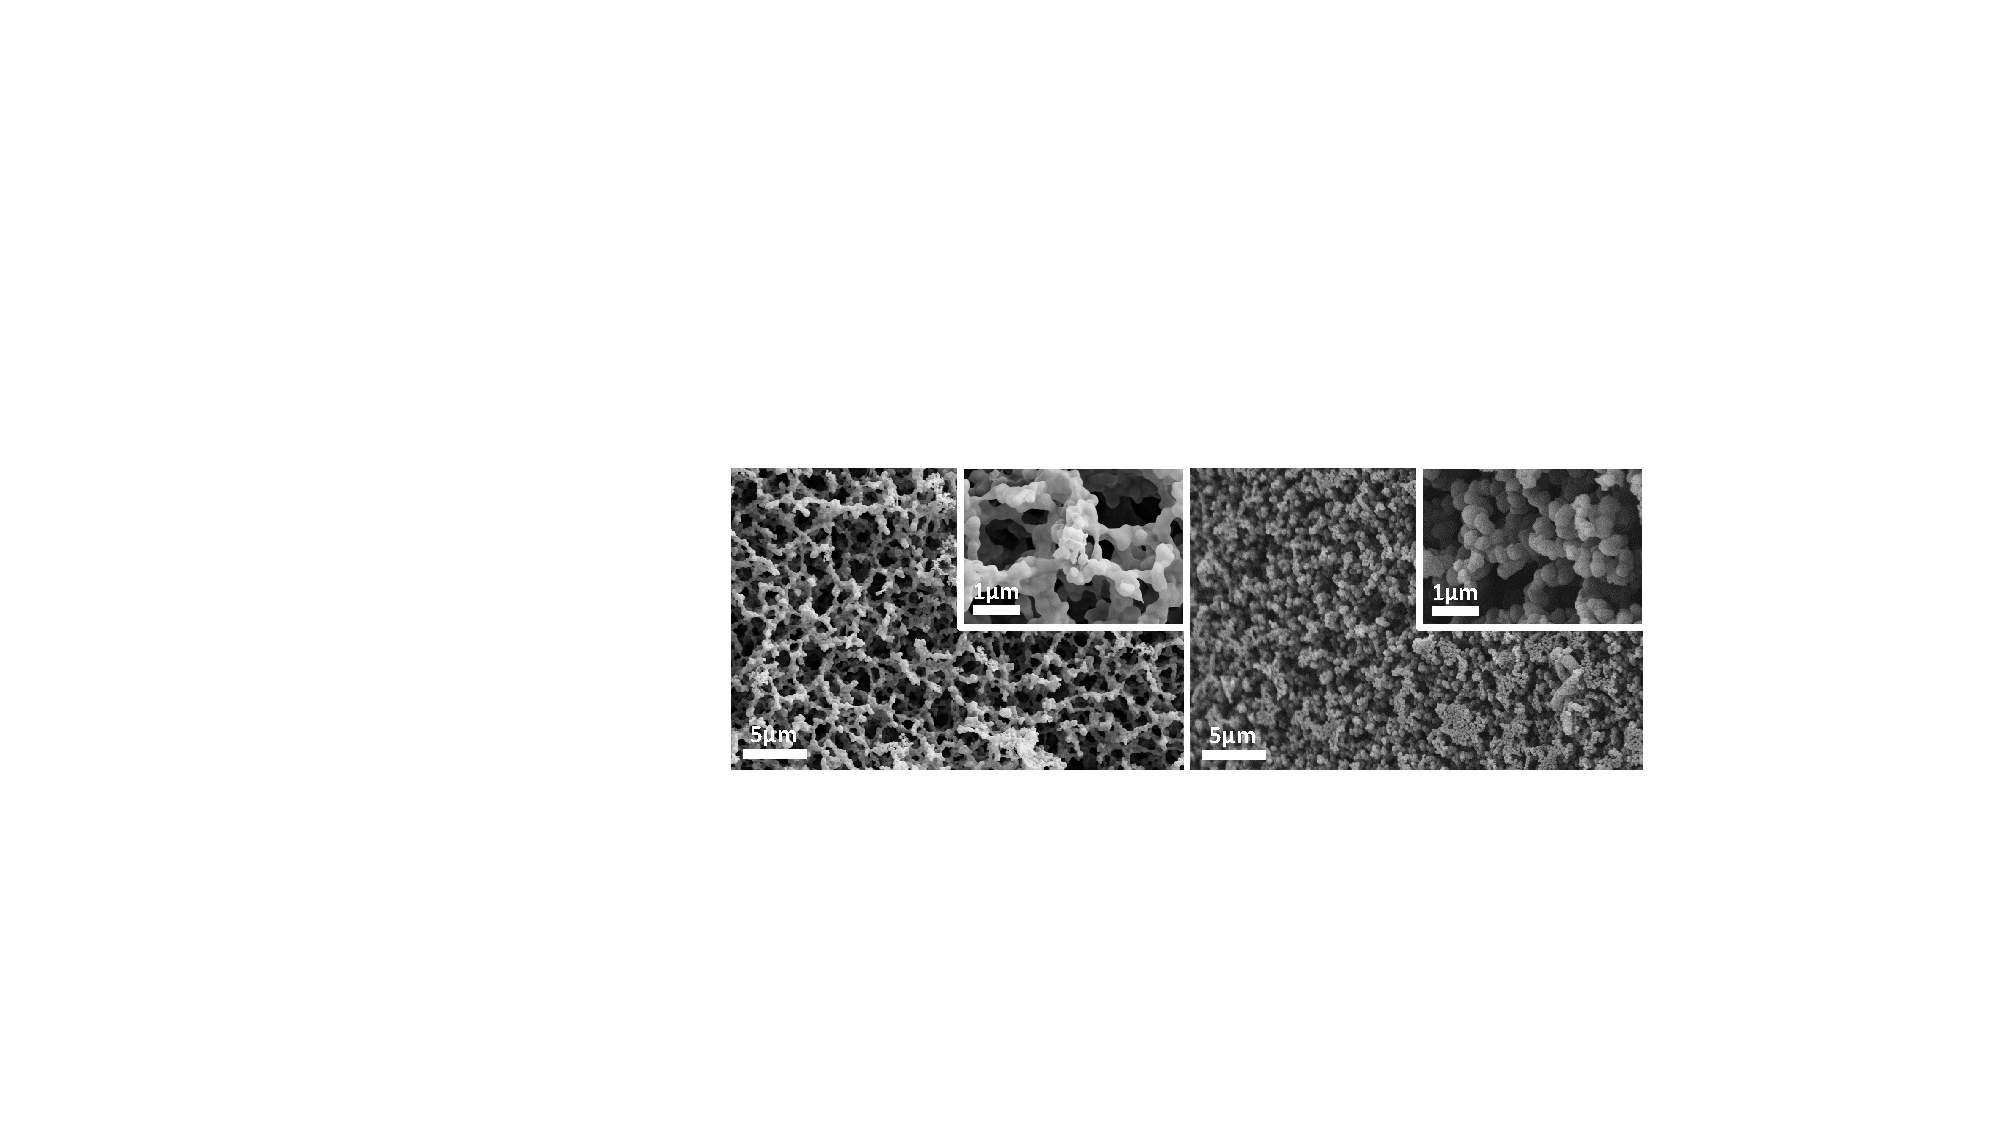
\includegraphics[width=\textwidth]{poreDeformation.pdf}
      \caption[SEM images of the HG03 hydrogel]{SEM images of the HG03 hydrogel ($\phi_w$) in swollen state (left) and shrunken state (right).}
      \label{fig:poreDeformation}
\end{figure*}

\section{Studying the effect of freeze-thaw method on the pore structure and response of the hydrogel}
Based on our prior experience, a freeze-thaw post-treatment with conventional closed-pore PNIPAAm gels (prepared in pure DMSO) results in enhanced swelling performance since the ice crystals can grow and expand or break the close-walled pore boundaries, resulting in a greater degree of pore interconnectivity (Figure~\ref{fig:freeze}). However, with the open-porous PNIPAAm gel (HG03), as the SEM images in Figure~\ref{fig:freeze1} shows, the as-prepared HG03 gel and the gel freeze-thawed 5 times in a $-20^{o}C$ freezer do not show a significant difference in their pore structures.

\begin{figure*}[!th]
      \centering
      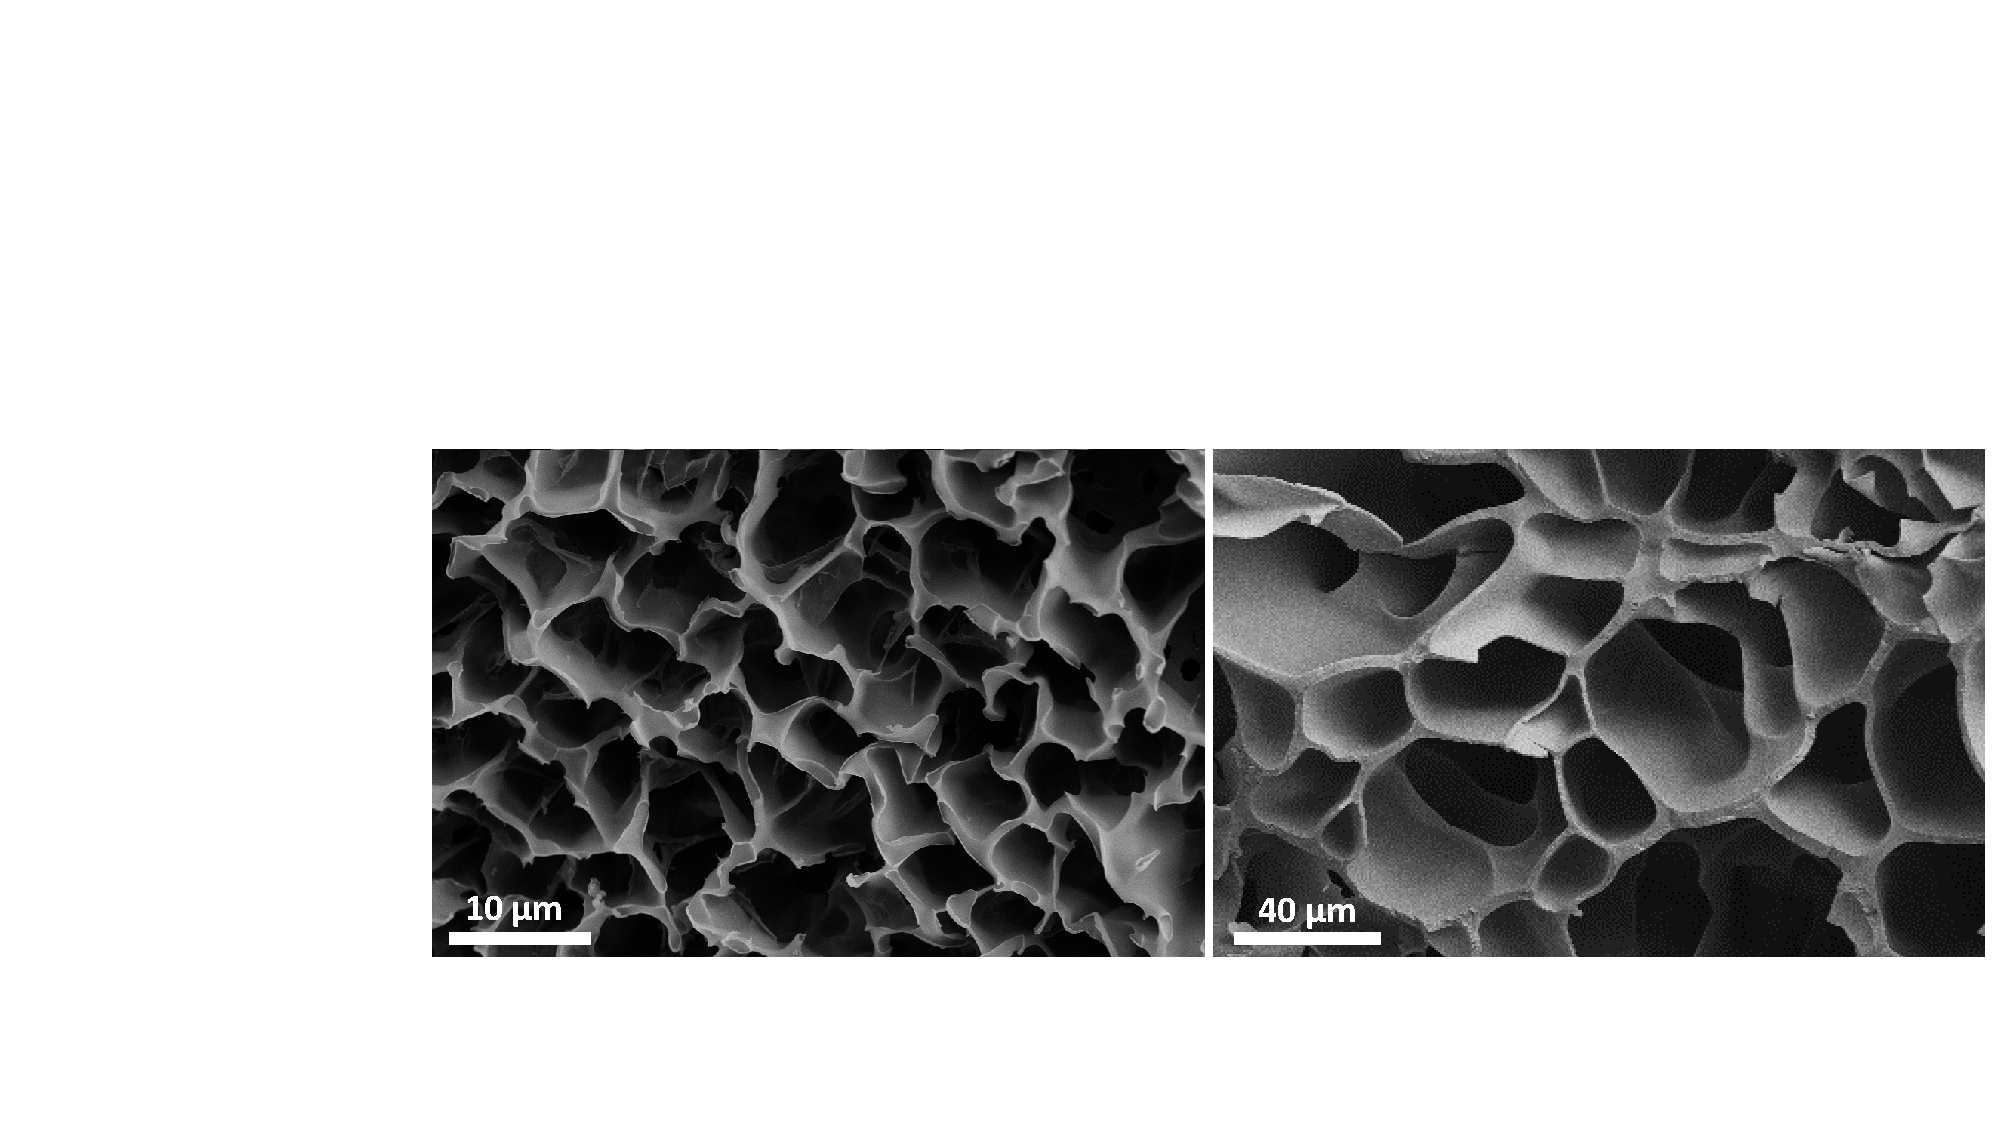
\includegraphics[width=\textwidth]{freeze.pdf}
      \caption[SEM images of as-prepared HG00]{SEM images of as-prepared HG00 (left) and HG00 after a single freeze-thaw cycle (right). scale bars inside the figures are different.}
      \label{fig:freeze}
\end{figure*}

\begin{figure*}[!th]
      \centering
      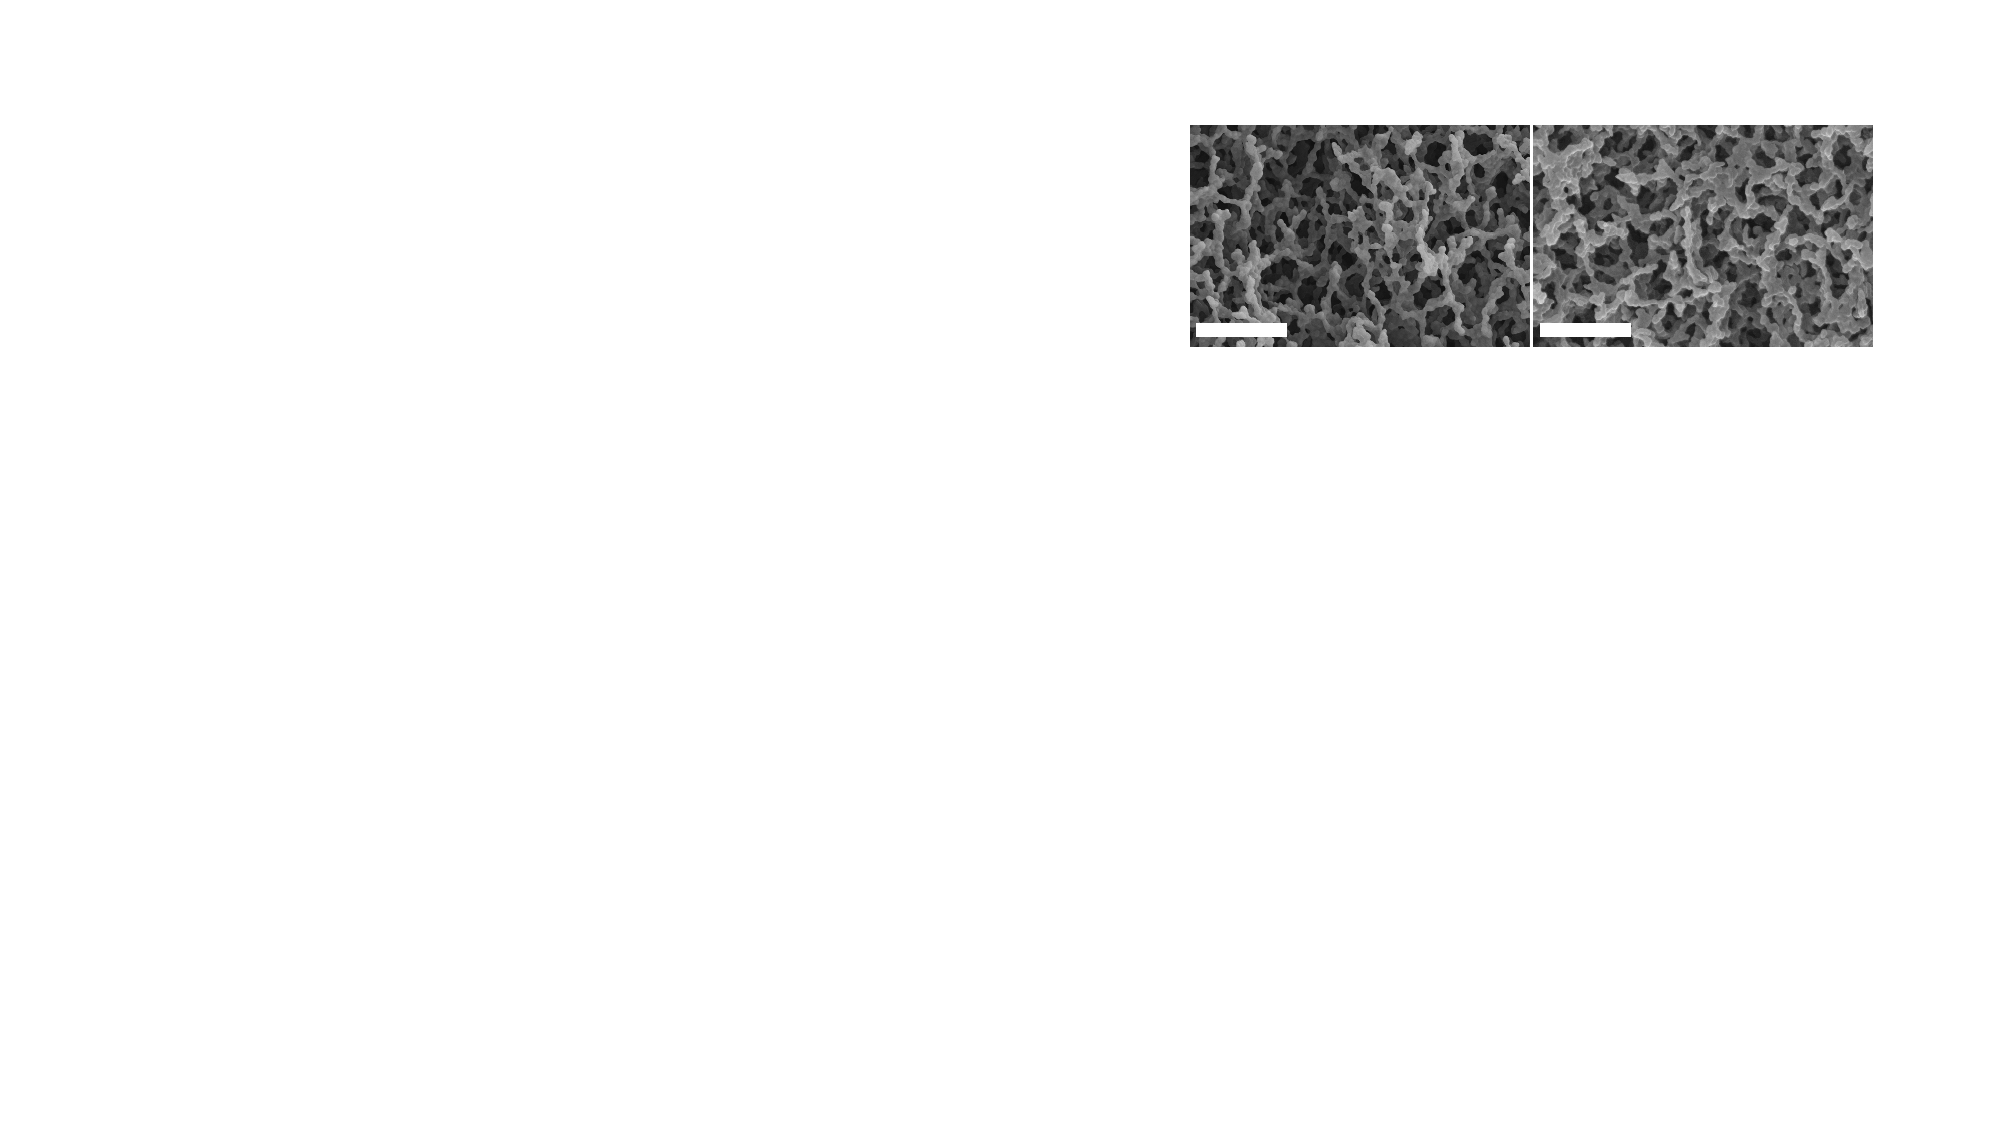
\includegraphics[width=\textwidth]{freeze1.pdf}
      \caption[SEM images of as-prepared HG03] {SEM images of as-prepared HG03 (left)  and HG03 hydrogels after five freeze-thaw cycles (right). scale bars: $5\mu$m.}
      \label{fig:freeze1}
\end{figure*}

\section{Comparing photopolymerization swelling performance to thermopolymerization}
The photopolymerized PNIPAAm sample is fabricated by dissolving $400~mg$~$mL^{-1}$ NIPAAm and $20~mg$~$mL^{-1}$ BIS into $2~mL$ of DMSO-water mixed solvent (0.27 vol fraction DMSO). $5\mu$L~$mL^{-1}$ of Darocur 1173 is added as the photoinitiator and vortexed thoroughly. The prepolymer solution is pipetted into a PDMS mold with dimensions $1~cm$$\times$$1~cm$$\times$$1.5~mm$ and illuminated with UV light for 15s to induce gelation. The photopolymerized PNIPAAm hydrogel is removed from the mold and allowed to soak in DI water for 24 hours to remove unreacted precursors and DMSO. The thermopolymerized PNIPAAm sample is fabricated by dissolving $400~mg$~$mL^{-1}$ NIPAAm and $20~mg$~$mL^{-1}$ BIS into $2mL$ of DMSO-water mixed solvent (0.27 vol fraction DMSO). $20~mg$~$mL^{-1}$ ammonium persulfate thermoinitiator is added, followed by vortexing until fully dissolved. This precursor is then chilled in a $-5^{o}C$ fridge for 15\,min, prior to adding $20~\mu$L~$mL^{-1}$ TEMED. After briefly inverting the precursor container several times to facilitate TEMED mixing, the precursor is pipetted into a PDMS mold with dimensions $1~cm$$\times$$1~cm$$\times$$1.5~mm$ and allowed to react for 15 hours. The thermopolymerized PNIPAAm hydrogel is removed from the mold and allowed to soak in DI water for 24 hours to remove unreacted precursors and DMSO.
To confirm that thermopolymerized PNIPAAm synthesized under these reaction conditions serves as an adequate control for the photopolymerized PNIPAAm, the reaction conversion is measured. The conversion quantifies how much of the dissolved precursor is consumed in the polymerization reaction, and is defined as follows, where W_dry  is the weight of the dry hydrogel, C_solute  is the total concentration of dissolved monomer and crosslinker, and V_mold  is the volume of the hydrogel mold:
\begin{align}
	Conversion = \frac{W_{dry}}{(C_{solute}×V_{mold} )}\times~100
\end{align}

Additionally, water content is measured to further validate that the thermopolymerized PNIPAAm synthesized under the above conditions serves as a comparable control. 
\begin{align}
	Water~Content = \frac{(W_{wet}-W_{dry})}{W_{wet}}\times~100
\end{align}

The matching conversion and water content for the photopolymerized and thermopolymerized PNIPAAm hydrogels indicate that the two can be compared directly.

\section{Effect of environmental conditions on SVA performance}
We have studied the effect of environment temperature on SVA performance by measuring the SVA force as the temperature of the water bath is varied. Figure~\ref{fig:envTemp} shows the SVA force as it is turned on for 60 s and off for 60 s for a total of 10 cycles.
\begin{figure*}[!ht]
      \centering
      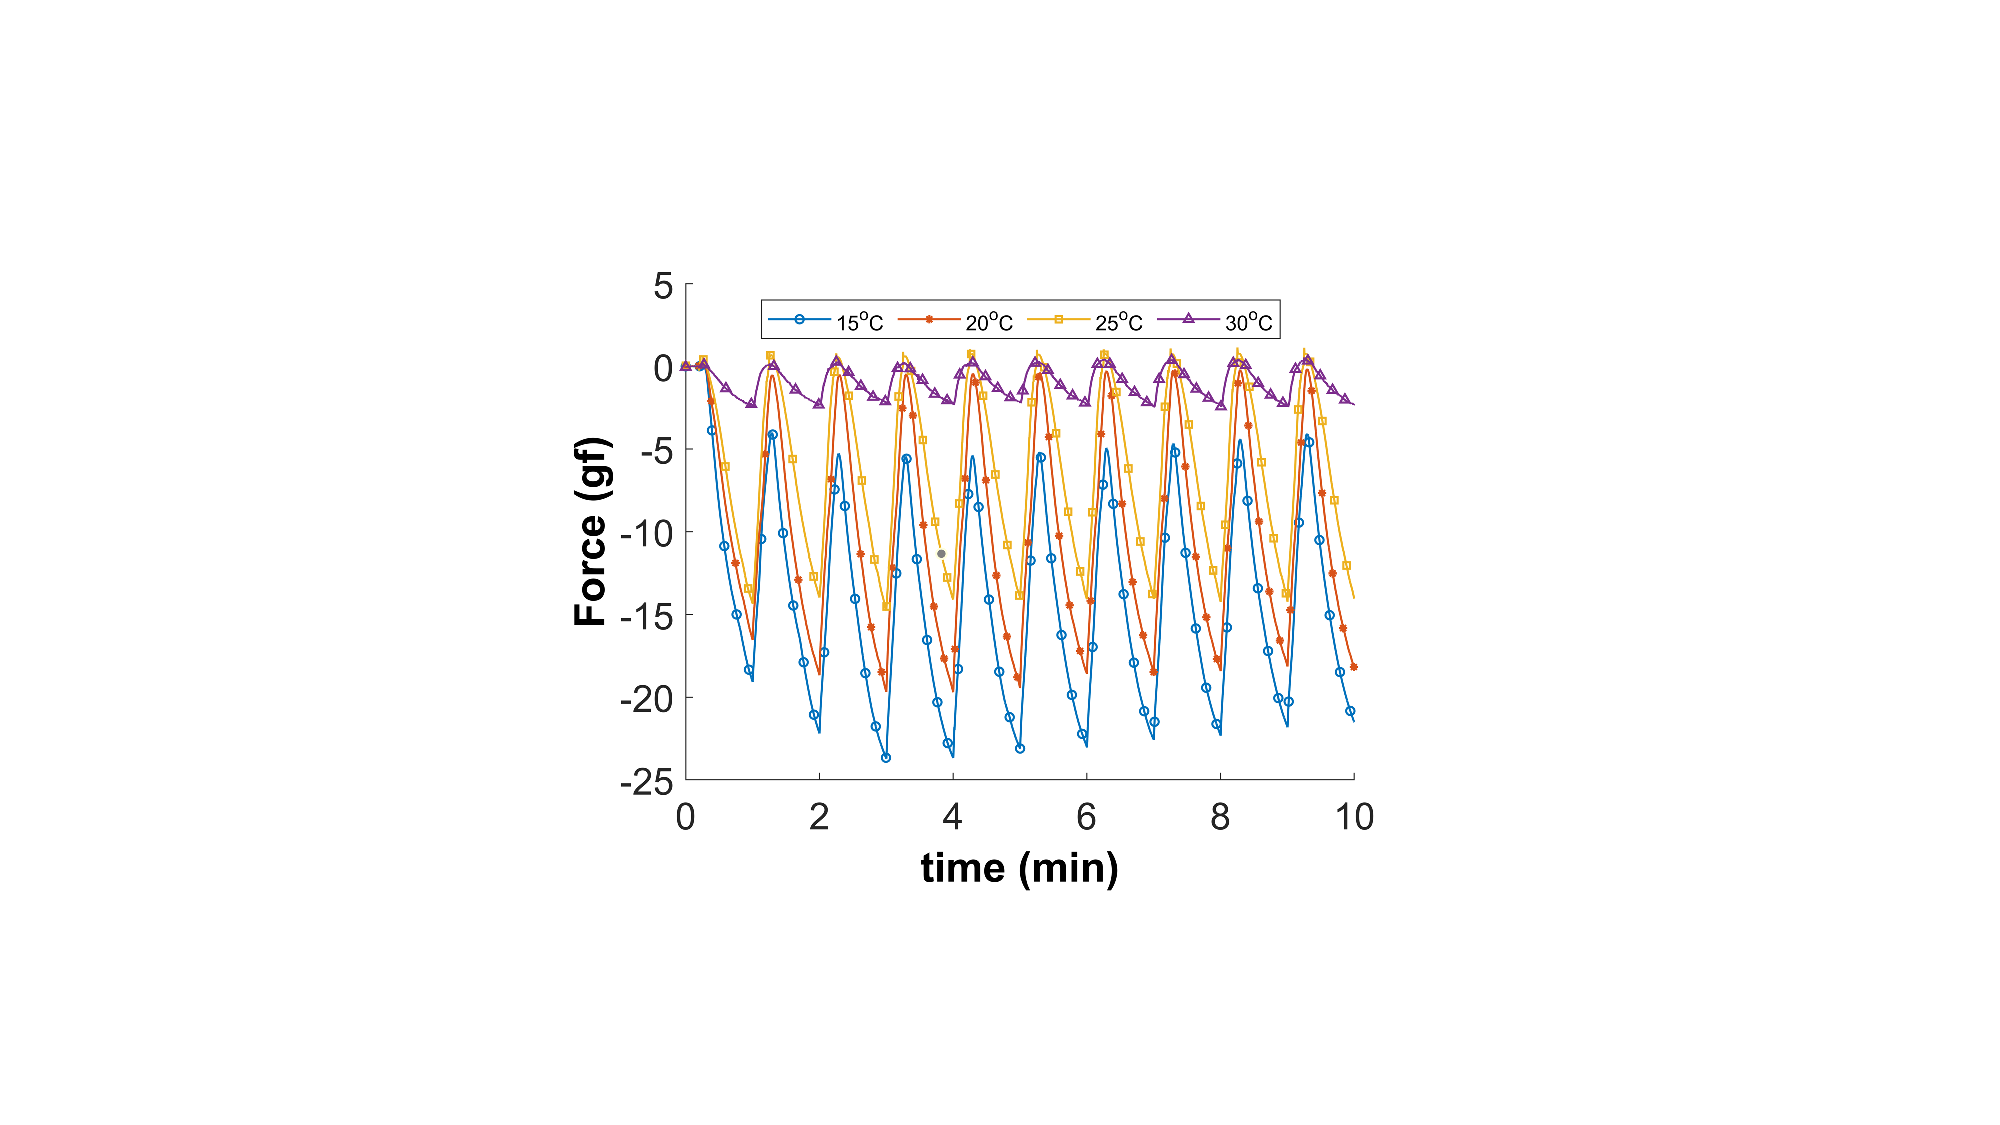
\includegraphics[width=0.8\textwidth]{envTemp.pdf}
      \caption[Effect of environment temperature]{Effect of the temperature of the water bath on the force production capacity of the SVAs.}
      \label{fig:envTemp}
\end{figure*}

\section{Cyclic tests}
We have characterized the long-term performance of the SVAs as they go through multiple cycles of expansion/contraction. The SVAs used for this test have not been gone through any heating and cooling cycles prior to this test. Figure~\ref{fig:cyclicDisp} shows the displacement over 1000 cycles. The temperature change dynamics is also measured by placing a thermocouple inside the SVA. As can be seen, the amplitude of the force is almost the same throughout the time. There is a very small drift which can be related to the settling of the force sensor setup over time. To further evaluate this, the SVA force in the first cycle is plotted against the last cycle. There is a slight improvement in the amplitude of the force and the SVA response seems to be slightly faster. We think this is due to the removal of residual DMSO, monomer and non-crosslinked polymer molecules from the gel when it is initially actuated. Overall, the SVAs does not show significant change in their performance over cyclic loads. 
\begin{figure*}[!htb]
      \centering
      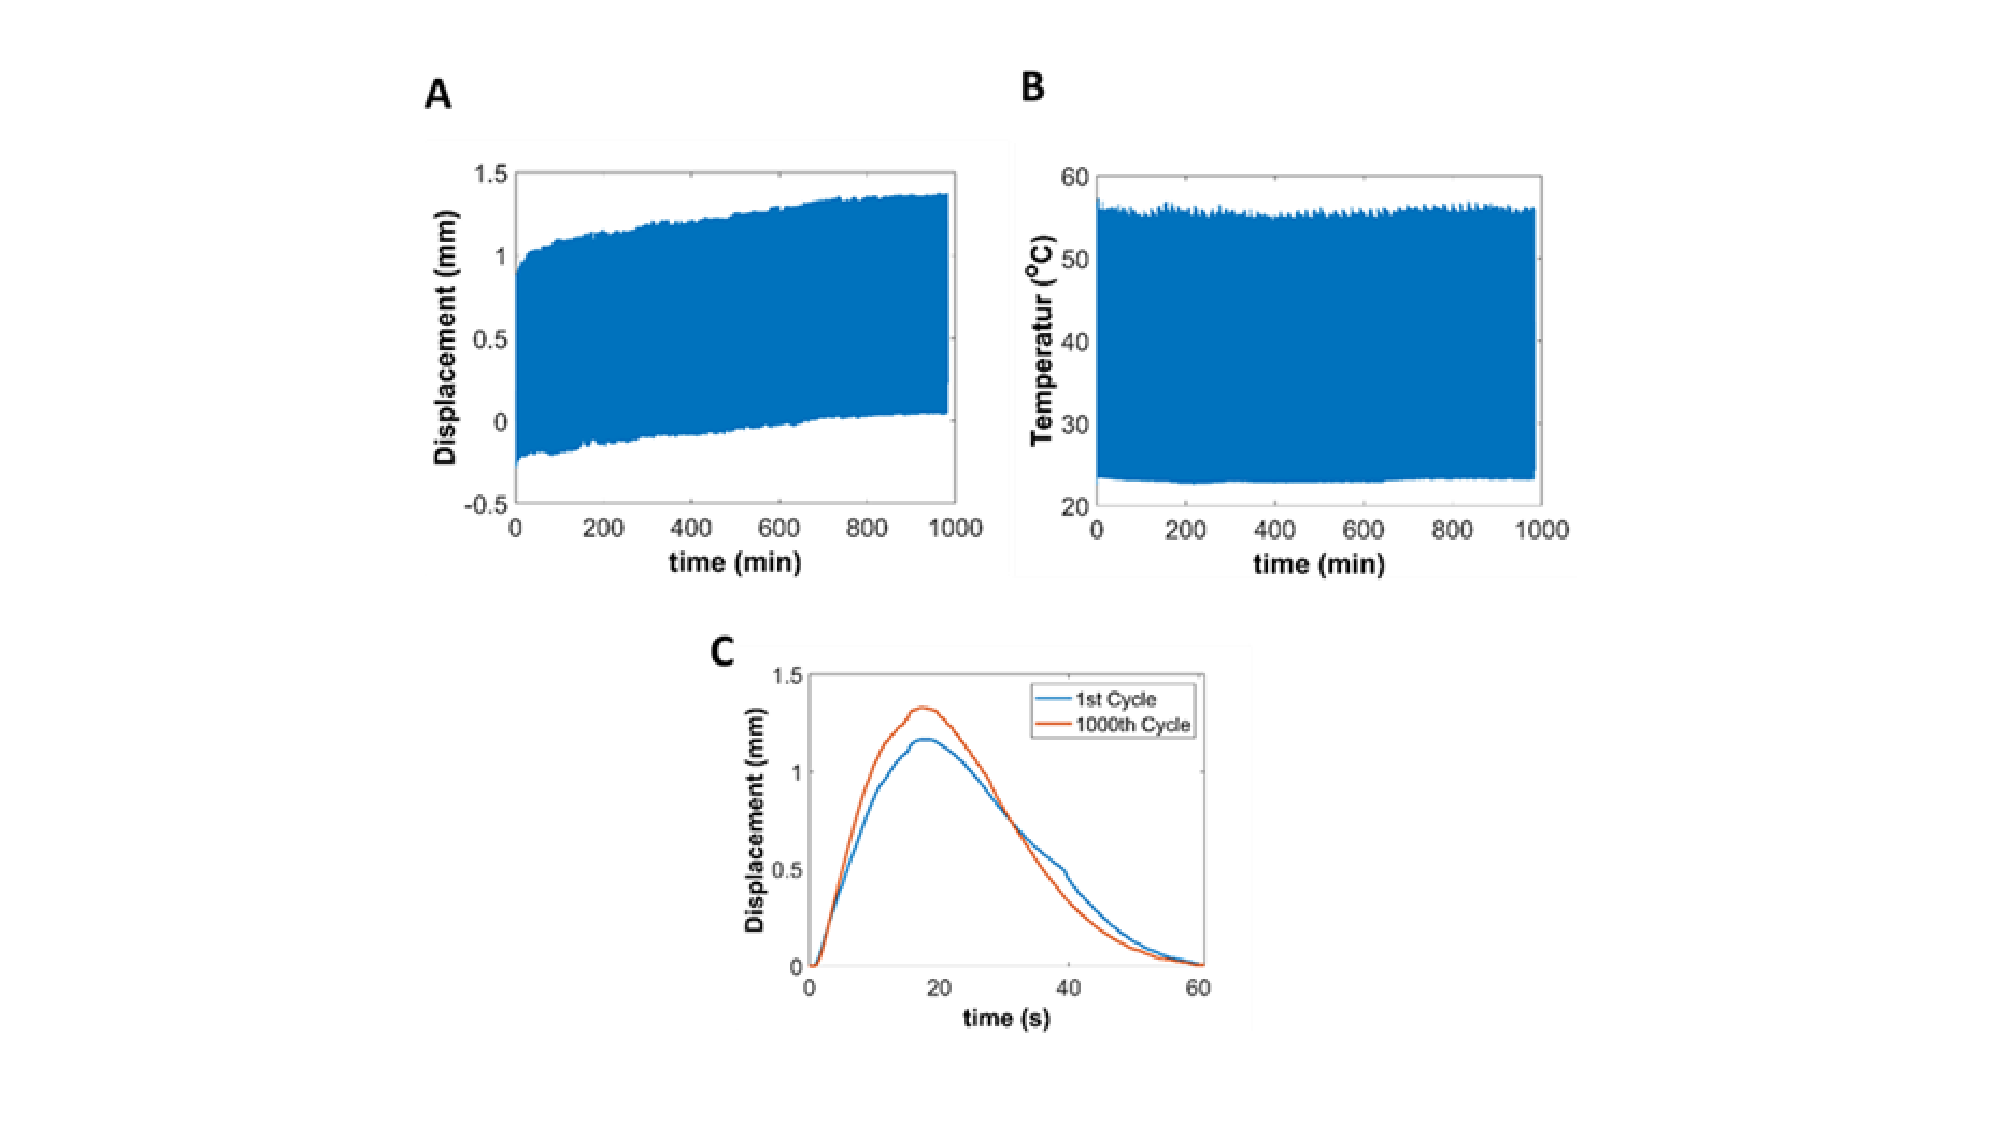
\includegraphics[width=0.8\textwidth]{cyclicDisp.pdf}
      \caption[Cyclic actuation of SVAs]{\textbf{Cyclic actuation of SVAs} A) Displacement of SVA over 1000 activation cycles. B) The temperature inside the SVA is also plotted. C) the displacement during first cycle and last cycle plotted for comparison.}
      \label{fig:cyclicDisp}
\end{figure*}

\section{Dependency of the performance of SVAs on their size}
As the volume change of hydrogel depends on temperature, the larger the size of the SVAs are, more time is needed for them to heat up by the Joule heaters and reach their minimum shrunken volume. To quantify this, we have tested 3 SVAs with different sizes and measured the displacement produced as the heater is turned on for 60 s and off for 60 s for a total of 10 cycles. As can be seen in Figure~\ref{fig:svaSize}, the larger SVAs produced higher deformation, however they need more time to reach that deformation. 
\begin{figure*}[!htb]
      \centering
      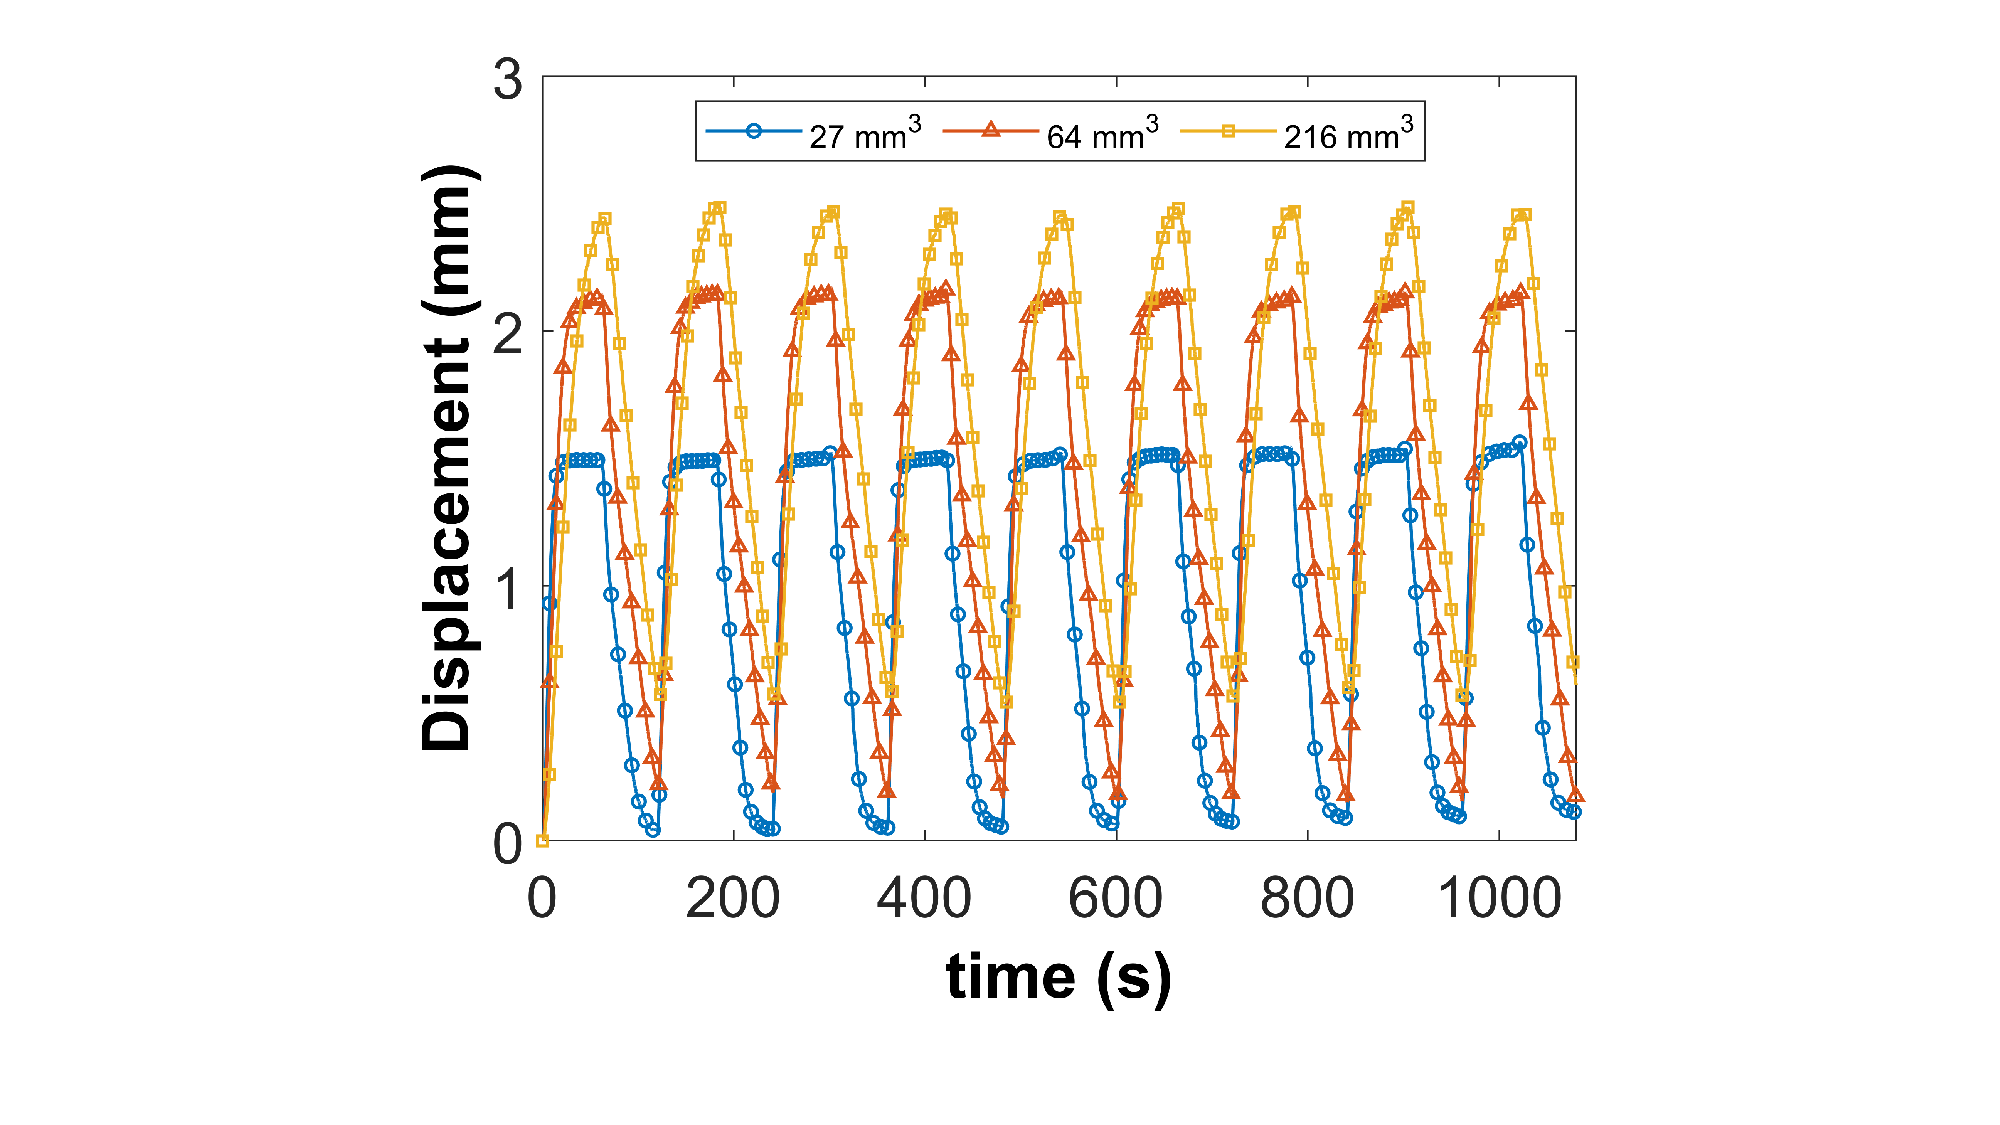
\includegraphics[width=0.6\textwidth]{svaSize.pdf}
      \caption[Effect of SVA size]{The effect of SVA size on the displacement produced as the heater is activated for 10 cycles.}
      \label{fig:svaSize}
\end{figure*}

\section{Kinetics of temperature change} 
In order to quantify the temperature of an SVA, a thermocouple is placed inside a SVA made of H03, close to the Joule heater as shown in Figure~\ref{fig:tempKinetics}. The temperature and displacement profiles as the heater is turned on for 15~s and then turned and kept off for 45~s are plotted for comparison.

\begin{figure}[!htb]
\centering
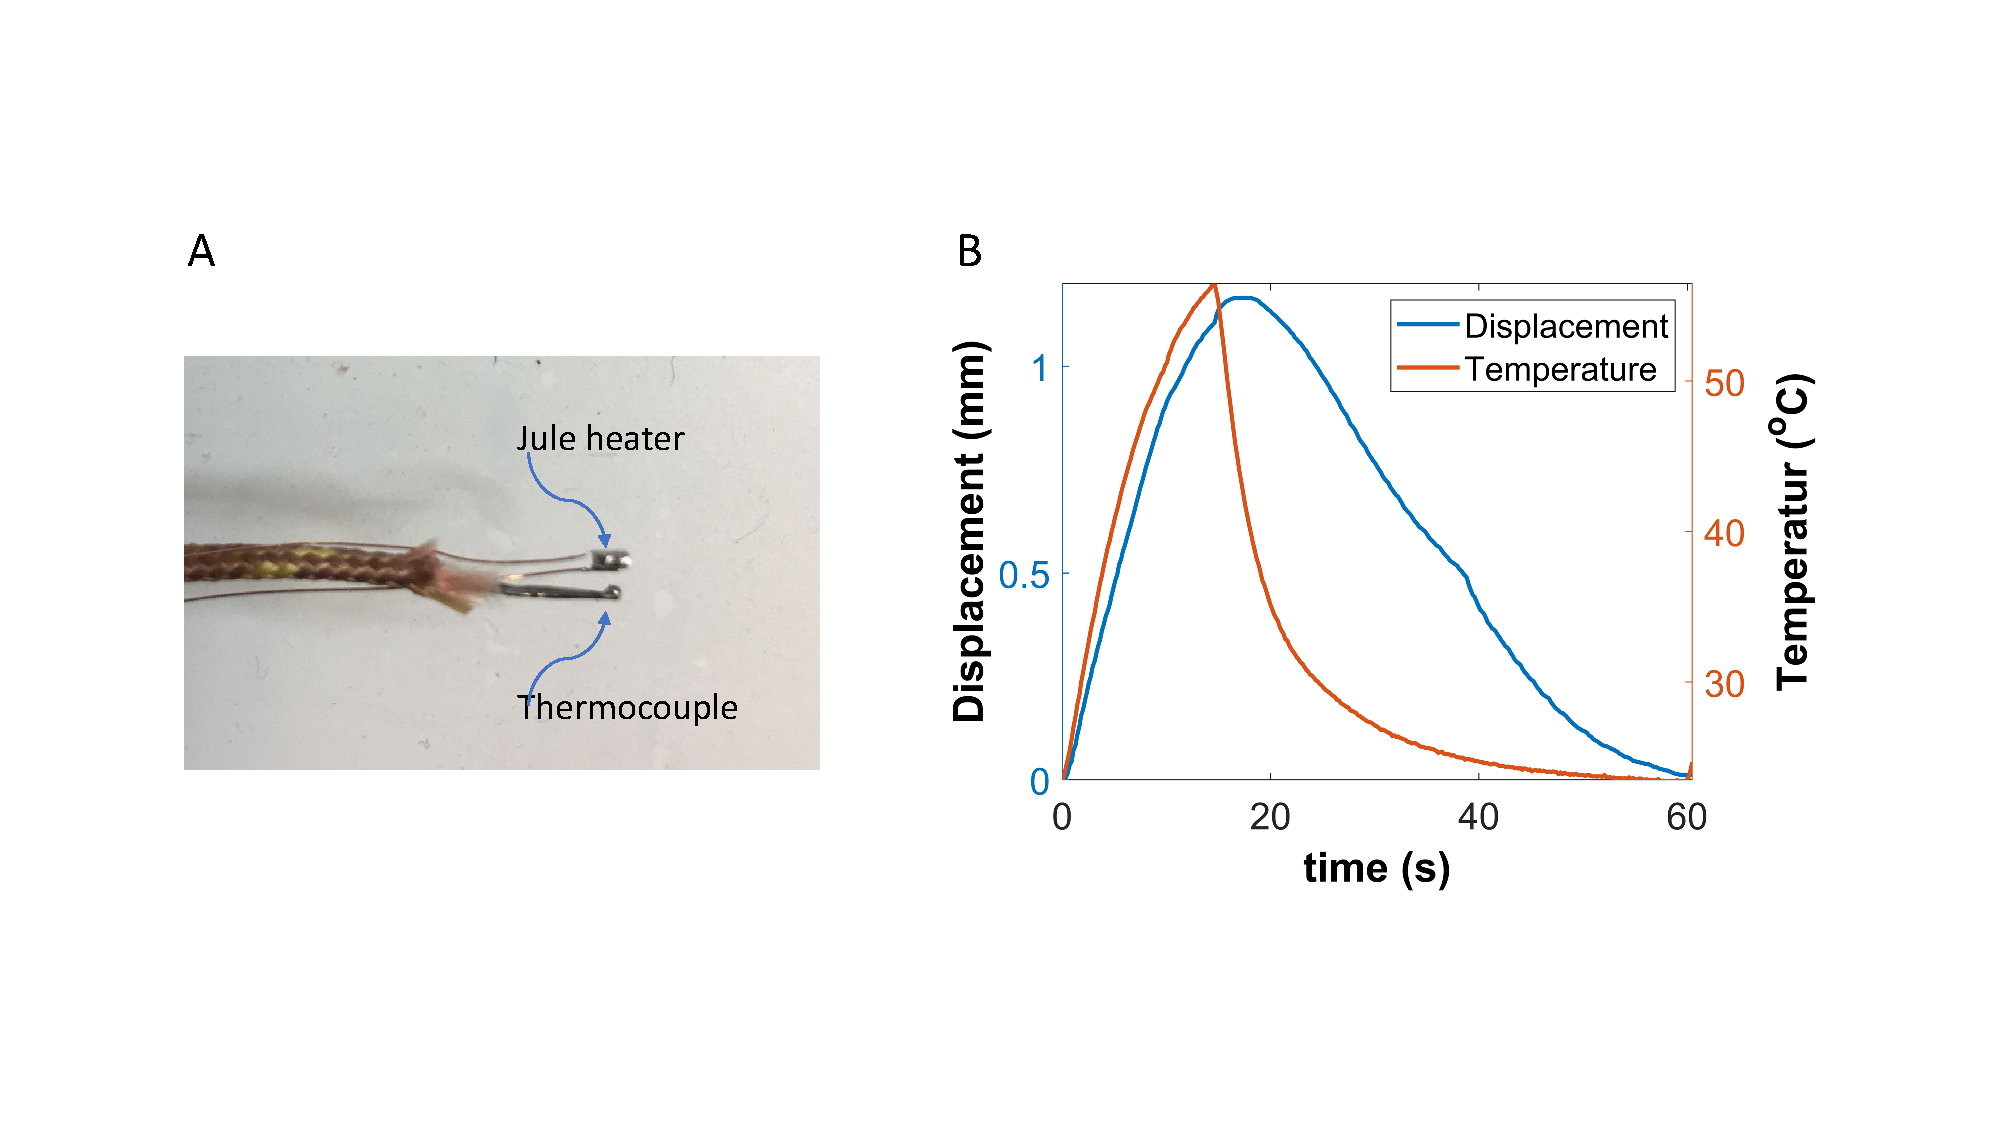
\includegraphics[width=\textwidth]{tempKinetics.pdf}
    \caption[Temperature kinetics in SVA actuation]{\textbf{Temperature kinetics in SVA actuation} A) a thermocouple is placed inside a SVA to measure the kinetics of the temperature change. B) temperature and displacement profiles }
    \label{fig:tempKinetics}
\end{figure}

%\begin{figure*}[!htb]
      %\centering
      %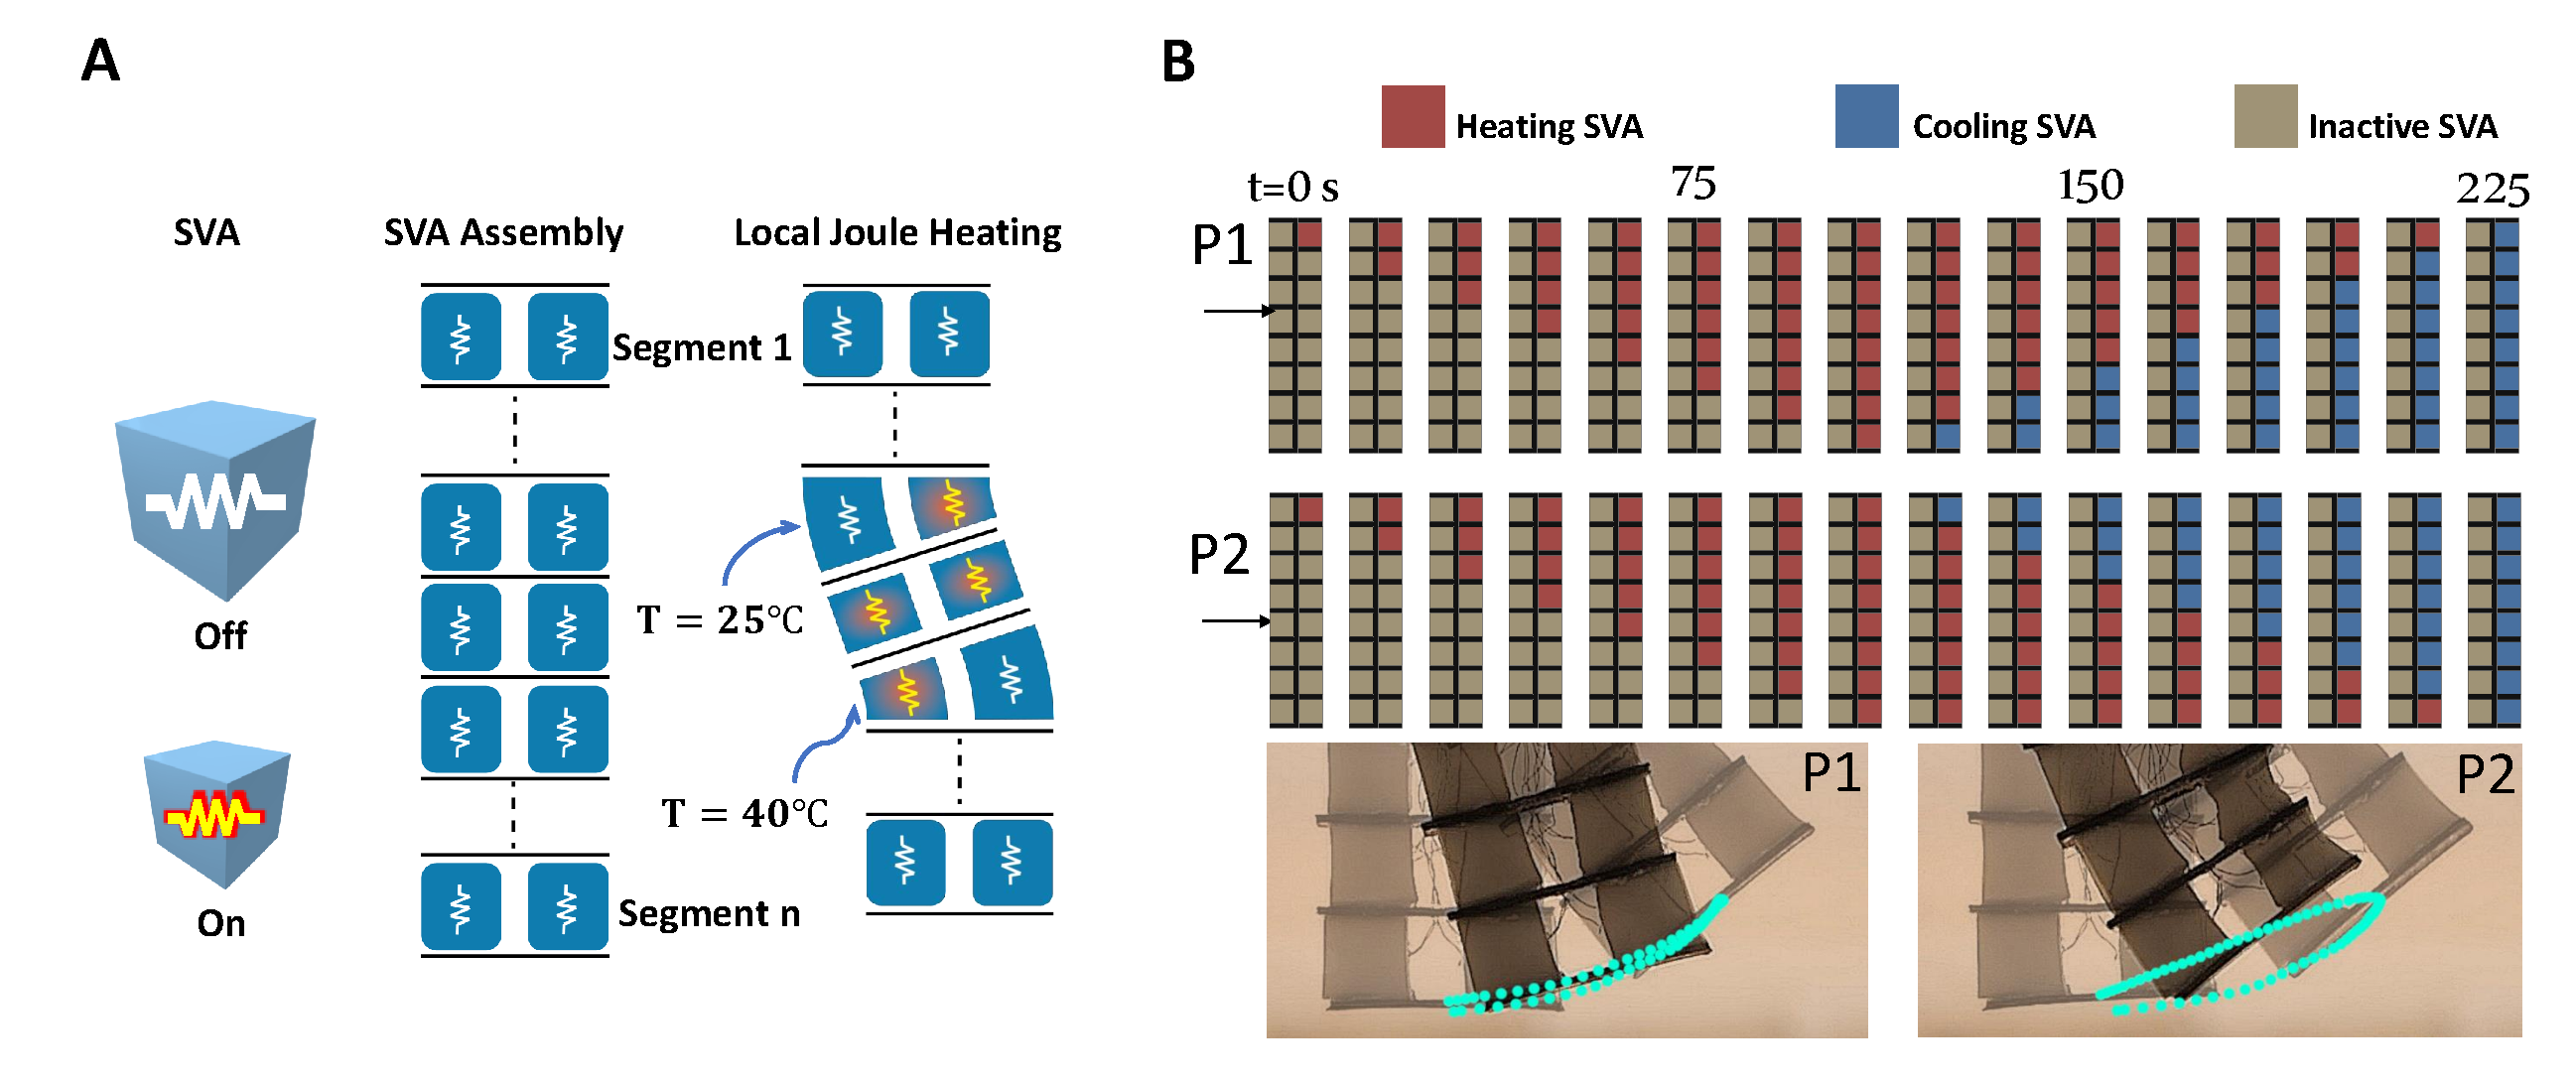
\includegraphics[width=\textwidth]{Fig2.pdf}
      %\caption{A) On and off states of a SVA is shown on the left column. Schematic of an assembly of SVAs is shown on the middle column. Activation of SVAs results in local increase in the temperature which leads to deformations that control the overall motion of the manipulator (right column). B) Sequentially activating SVAs 1 through 8 according to the patterns labeled P1 and P2 results in different trajectories followed by the tip of the manipulator (shown in cyan at the bottom). For details, see Movie S1.}
      %\label{fig:treajectory}
   %\end{figure*}